\documentclass[a4paper]{article}                         %文章类别
%--------------------------------------------------调用宏包--------------------------------------------------%
\usepackage{graphicx}                           %Required for inserting images
\usepackage{ctex}                               %用于设置中文编译环境
\usepackage{titlesec}
\usepackage{microtype}                          %控制表格打印高度
\usepackage{multirow}                           %表格多行填写文本
\usepackage{booktabs,makecell,multirow,tabularx}%表格多行填写文本
\usepackage{indentfirst}                        %用于设置首行缩进
\usepackage{booktabs}                           %用于设置三线表的线的宽度
\usepackage{float}
\usepackage[export]{adjustbox}                  %用于调整pdf的大小宽度
\usepackage{listings}                           %用于插入代码的包
\usepackage{xcolor}                             %用于设置代码颜色
\usepackage{hyperref}                           %用于引用网站的包 
%--------------------------------------------------定义代码的样式--------------------------------------------------%
\lstset{
  language=C++,                   % 代码语言
  basicstyle=\ttfamily,            % 代码的基本样式,\ttfamily 表示等宽字体
  keywordstyle=\color{blue},       % 关键词颜色
  commentstyle=\color{green!50!black}, % 注释颜色
  stringstyle=\color{red},         % 字符串颜色
  numbers=left,                    % 在左边显示行号
  numberstyle=\tiny\color{gray},   % 行号的样式
  stepnumber=1,                    % 行号的步长
  tabsize=2,                       % 制表符宽度
  showspaces=false,                % 不显示空格
  showstringspaces=false,          % 不显示字符串中的空格
  breaklines=true,                 % 自动换行
  breakatwhitespace=false,         % 仅在空格处换行
  frame=single,                    % 用框架框住代码
  backgroundcolor=\color{gray!10}  % 背景颜色
}

          
\titleformat{\section}                          %section部分格式设置
{\centering\Large\bfseries}{\thesection}{1em}{}

\setlength{\parindent}{10em}                    %2em代表首行缩进两个字符


\title{Proj_{1}}       %文章标题

\date{}                                         %日期
\author{}

\begin{document}                                %全文开始

\maketitle

%--------------------------------------------------正文----------------------------------------------------%
\section{解题思路}        
    \subsection{问题简介}
        \subsubsection{SAT问题}
            本问题称为``布尔表达式可满足性问题'',英文术语为``Boolean Satisfiability Problem'',该术语的Abbreviation是``SAT'' \par
                我们需要\textbf{解决的问题}是:对于一个布尔表达式(该布尔表达式由m个clause通过``$\cap$''组成,即$clause_{1} \cap \cdots \cap clause_{m}$),能否找到一组真值,使得该布尔表达式的赋值为真(即所有的$clause_{i}$都为true)\par
                拿一个简单的例子进行说明,现在我们考虑只有n=3个变量和m=1个clause的布尔表达式:

            \begin{center}
                $x_{1} \cup \overline{x_{2}} \cup x_{3}$
            \end{center}

            \par
            我们只需令:
        
            \begin{center}
                $x_{1}$ = true \quad $x_{2}$、$x_{3}$ 任意取
            \end{center}
            
            \par
            那么,该布尔表达式就为true
            \par
            一般地, 对于有n个变量和m个clause的布尔表达式:

            \begin{center}
                $clause_{1} = x_{1} \cup x_{2} \cup \cdots \cup x_{i} \cup \cdots \cup x_{n}$
            \end{center}
            
            \begin{center}
                $\vdots$
            \end{center}

            \begin{center}
                $clause_{l} = x_{1} \cup \overline{x_{2}} \cup \cdots \cup x_{i} \cup \cdots \cup x_{n}$
            \end{center}

            \begin{center}
                $\vdots$
            \end{center}

            \begin{center}
                $clause_{m} = x_{1} \cup \overline{x_{2}} \cup \cdots \cup \overline{x_{i}} \cup \cdots \cup x_{n}$
            \end{center}


            \par
            我们能不能找到一组真值,使得该布尔表达式的赋值为真呢?
            \par
            这就是我们接下来要讨论的``SAT''问题
        \subsubsection{K-SAT问题}
            那么什么是``K-SAT问题''呢?\par
                从定义上来讲,就是说我们使得布尔表达式中的每个clause只出现k个变量,我们拿一个其中一个$clause_{l}$进行说明:

        \begin{center}
            $clause_{l}=x_{1} \cup x_{2} \cup \cdots \cup x_{i} \cup \cdots \cup x_{j}$
        \end{center}

        \noindent{其中:}\par
            这个$clause_{l}$中出现的变量个数一共有k个,即$x_{1}\cdots x_{i} \cdots x_{j}$一共有k个\par
            这是什么意思呢?同样,我们拿一个简单的例子进行说明,考虑有n=5个变量和m=3个clause的布尔表达式:

        \begin{center}
            $x_{1} \cup \overline{x_{2}} \cup \overline{x_{3}} \cup x_{5}$
        \end{center}

        \begin{center}
            $x_{1} \cup x_{2} \cup x_{3} \cup x_{4}$
        \end{center}

        \begin{center}
            $x_{1} \cup x_{3} \cup x_{4} \cup x_{5}$
        \end{center}

        我们可以注意到一个事实:\\
        \begin{center}
            每个clause中出现的变量个数只有4个
        \end{center}
        \par
        很自然地,我们现在会有下面几个问题:\\
        \begin{center}
            我们不是已经定义了这个布尔表达式有n=5个变量吗?
        \end{center}
        \begin{center}
            为什么这个clause中出现的变量个数是4呢?
        \end{center}
        \begin{center}
            这个`4'代表了什么意思呢?
        \end{center}
            \par
        我们现在来进行回答:这个`4'实际上是``K-SAT问题''当中的K,换言之,在我们刚刚举的例子中,我们令K=4,也就是说,这是一个``K=4-SAT问题'',即``4-SAT问题''
        \subsubsection{3-SAT问题}
        同样,很自然地,我们回到要求解的问题当中,我们对给出的测例进行观察:

        \begin{center}
            $x_{1} \cup \overline{x_{2}} \cup \overline{x_{4}}$
        \end{center}

        \begin{center}
            $x_{2} \cup \overline{x_{3}} \cup x_{4}$
        \end{center}
        \begin{center}
            $x_{2} \cup x_{3} \cup x_{4}$
        \end{center}
        \begin{center}
            $x_{2} \cup x_{3} \cup \overline{x_{4}}$
        \end{center}
        \par
        我们可以注意到一个事实:\\
        \begin{center}
            每个clause中出现的变量个数只有3个
        \end{center}
        \par
        也就是说,我们需要解决的问题是一个``3-SAT问题''\\
        那么,如何进行求解呢?通过查询资料(已放在``参考文献''处),我们给出如下几种经典的解决方案:\par
            (1)回溯法 —— 最初尝试方式\par
            (2)DPLL算法 —— 主要实现方式\par
            (3)WalkSAT算法 —— 未尝试进行实现\\
        我们将在``解题方法简介''中进行解释
    \subsection{解题方法简介}
        ``SAT问题''的求解方法有很多,
        主要分为\underline{\textbf{完备性算法}}和非完备性算法,
        很自然地,我们会有两个问题:\\
        \begin{center}
            什么是``\underline{\textbf{完备性算法}}''?
        \end{center}
        \begin{center}
            什么是``非完备性算法''?
        \end{center}
        \par
        不太严谨地,我们拿一个例子进行说明:考虑有一张银行卡,它的密码有6位数字,但我们现在忘掉了它的密码,那么我们应该怎样试出这个银行卡的密码呢?\par
        很自然地,我们会有两种主要的尝试方案(不考虑其他外界因素):\\
        \begin{center}
            一个一个排列组合进行尝试
        \end{center}    
        \begin{center}
            灵光一现,想到一个密码,然后输入并且进行验证
        \end{center}
        \par
        我们认为:
        \begin{center}
            第(1)种方案是``完备的''
        \end{center}
        \begin{center}
            第(2)种方案是``不完备的''
        \end{center}
        \par
        我们现在来对这两个``尝试方案''进行分析\\
        针对``\underline{尝试方案1}'':\par
            通过对这6位密码进行排列组合一个一个进行尝试,我们肯定能找到一组数字,解开这个银行卡的密码\par
            回到我们要求解的问题上,也就是说,通过排列组合一个一个进行尝试,我们一定能找出一组解,使得该布尔表达式的赋值为真\par
            从本质上讲,``完备性算法''给我们一种``暴力枚举''的感觉\par
            很自然地,既然``完备性算法''给我们一种``暴力枚举''的感觉,那也就是说,这一类算法有一个非常显著的特点:\\
        \begin{center}
            一定能算 \quad 但是 \quad \textbf{慢}!
        \end{center}
        \par
        ``\textbf{慢}''这个特点我们会在``基于回溯法的实现''中体现出来(实际上确实慢,尤其是遇上数据量比较大的测例)\par
        同样,很自然地,我们会有这么一个问题:\\
        \begin{center}
            有没有方法让这个求解速度``快''起来呢?
        \end{center}
        我们来进行回答:\\
        \begin{center}
            我求解这个``3-SAT问题''的主要实现方法\ ——\ \underline{\textbf{DPLL算法}}
        \end{center}
        针对``\underline{尝试方案2}'':\par
            ``灵光一现''想起一个密码并输入进行验证\par
            同样,回到我们要求解的问题上,那么这里的``灵光一现''这是什么意思呢?\par
            同样,从本质上讲,``非完备性算法''给我们一种``搜索局部最优解''的感觉(实际上也确实是这样的)\par
            很自然地,既然``非完备性算法''给我们一种``搜索局部最优解''的感觉,也就是说,这一类算法也有一个非常显著的特点:\\
        \begin{center}
            \textbf{快}!
        \end{center}
        \par
        很自然地,我们会有这么一个问题:\\
        \begin{center}
            ``非完备性算法''这么``快'',会不会有某些问题呢?
        \end{center}
        \par
        我们这里不展开论述
        \subsubsection{回溯法}
        那么,什么是``回溯法''呢?首先,从``回溯法''当中的``回溯''上进行展开,``回溯''一般与``递归''联系在一起\par
            很自然地,我们自然会问:什么是``递归''呢?\par
        同样地,我们拿一个简单的例子进行说明:考虑``for loop''和``递归''\\
        我们认为:\par
            (1)``for loop''属于``横向遍历''\par
            (2)``递归''属于``纵向遍历''\\
        很自然地,我们会有这么两个问题:\par
            (1)什么是``横向遍历''呢?\par
            (2)什么是``纵向遍历''呢?\\
        下面我们进行解释:\\
        针对``for loop''当中的``\underline{横向遍历}'':\par
            我这里截取了``彻底搞懂回溯法''当中的``把回溯问题抽象为树形结构''当中的一张图来进行粗略地说明:

        \begin{figure}[H]
            \centering
            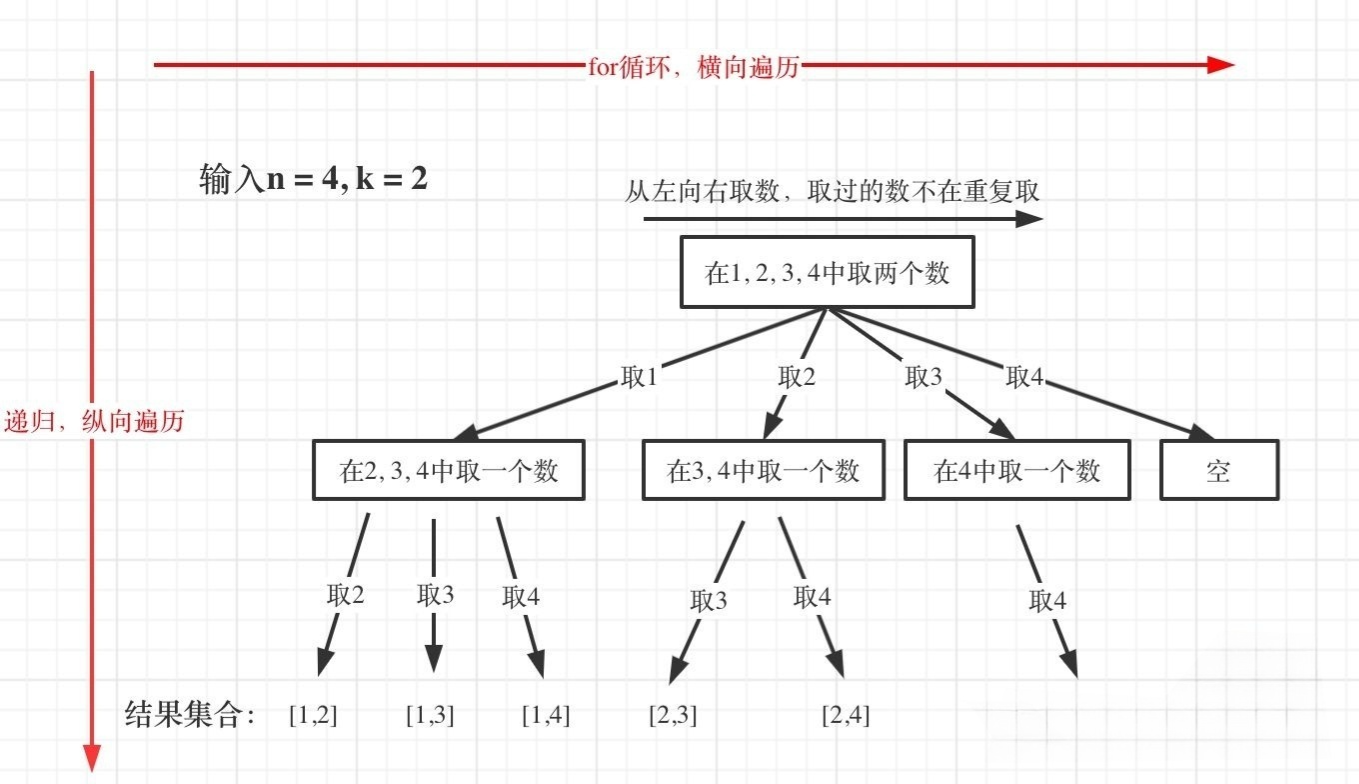
\includegraphics[width=10cm]{Figure/Figure_1.png}
            \caption{把回溯问题抽象为树形结构}
        \end{figure}
        \noindent
        针对``递归''当中的``\underline{纵向遍历}'':\par
            我这里截取了``HELLO Algo''里面``求和函数的递归过程''当中的一张图来进行粗略地说明:

        \begin{figure}[H]
            \centering
            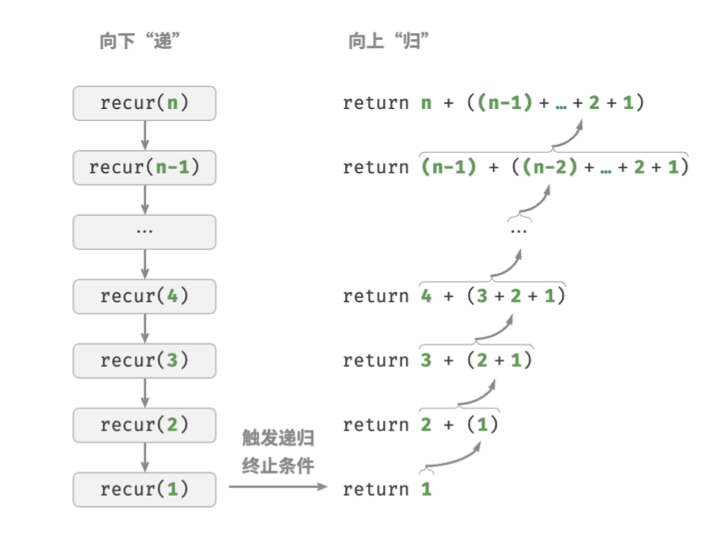
\includegraphics[width=10cm]{Figure/Figure_2.jpg}
            \caption{求和函数的递归过程}
        \end{figure}

        \noindent
        观察两张图示,我们可以非常清晰地认识到:\par
        ``回溯法''的本质就是一种``暴力搜索''
        (形式上与``for loop''类似,
        只不过一个是横向遍历,
        一个是纵向遍历而已,
        区别仅限于此)
        但我们之前在分析``回溯法''这一类``完备性算法''的时候,
        我们已经指出了``完备性算法''的一个非常大的问题 ——``\textbf{慢}''\par
            实际上,我在利用``回溯法''求解``3-SAT问题''的过程中,也确实遇到了这么个问题:\par
                (1)求解数据量比较少的测例基本没有问题\par
                (2)求解数据量比较大的测例基本上都是超时\\
            在``基于回溯法的实现''处,会展开论述这个问题\par
                很自然地,我去寻找另一类求解``3-SAT问题''的方法\ ——\ 基于``回溯法''的``DPLL算法'' \ —— \ 改进后的一种``完备性算法''
        \subsubsection{DPLL算法}
        那现在我们来重点介绍一下``\underline{\textbf{DPLL算法}}''!\par
        那么,到底什么是``DPLL算法''呢?查阅资料后,我们可以知道,所谓``DPLL算法'',
        是解决``SAT问题''的一种``完备性算法'',是对``回溯法''的一种改进。\\
        \newline
        \noindent
        这个算法主要由如下几个\textbf{核心阶段}组成:\par
            (1)当前子句可满足判断\ ——\ Current Clause Satisfied\par
            (2)布尔表达式可满足判断\ ——\ All Clauses Satisfied\par
            (3)空子句判断\ ——\ Has Empty Clause\par
            (4)单位子句传播\ ——\ Unit Propagation\par
            (5)孤立文字消去\ ——\ Pure Literal Elimination\par
            (6)使用DPLL算法(实际上就是``回溯法'')进行求解\\
        \par
        在这里做一个比较粗略的解释:
        ``DPLL算法''从本质还是``回溯法'',
        只不过我们对``回溯法''中处理``literal''的方式进行了各种优化,
        让这个``回溯法''变得更加切实可行
        \par
        关于``DPLL算法'',
        我们下面给出一张比较简略的流程图来对DPLL算法有一个比较粗略的了解:

        \begin{figure}[H]
            \centering
            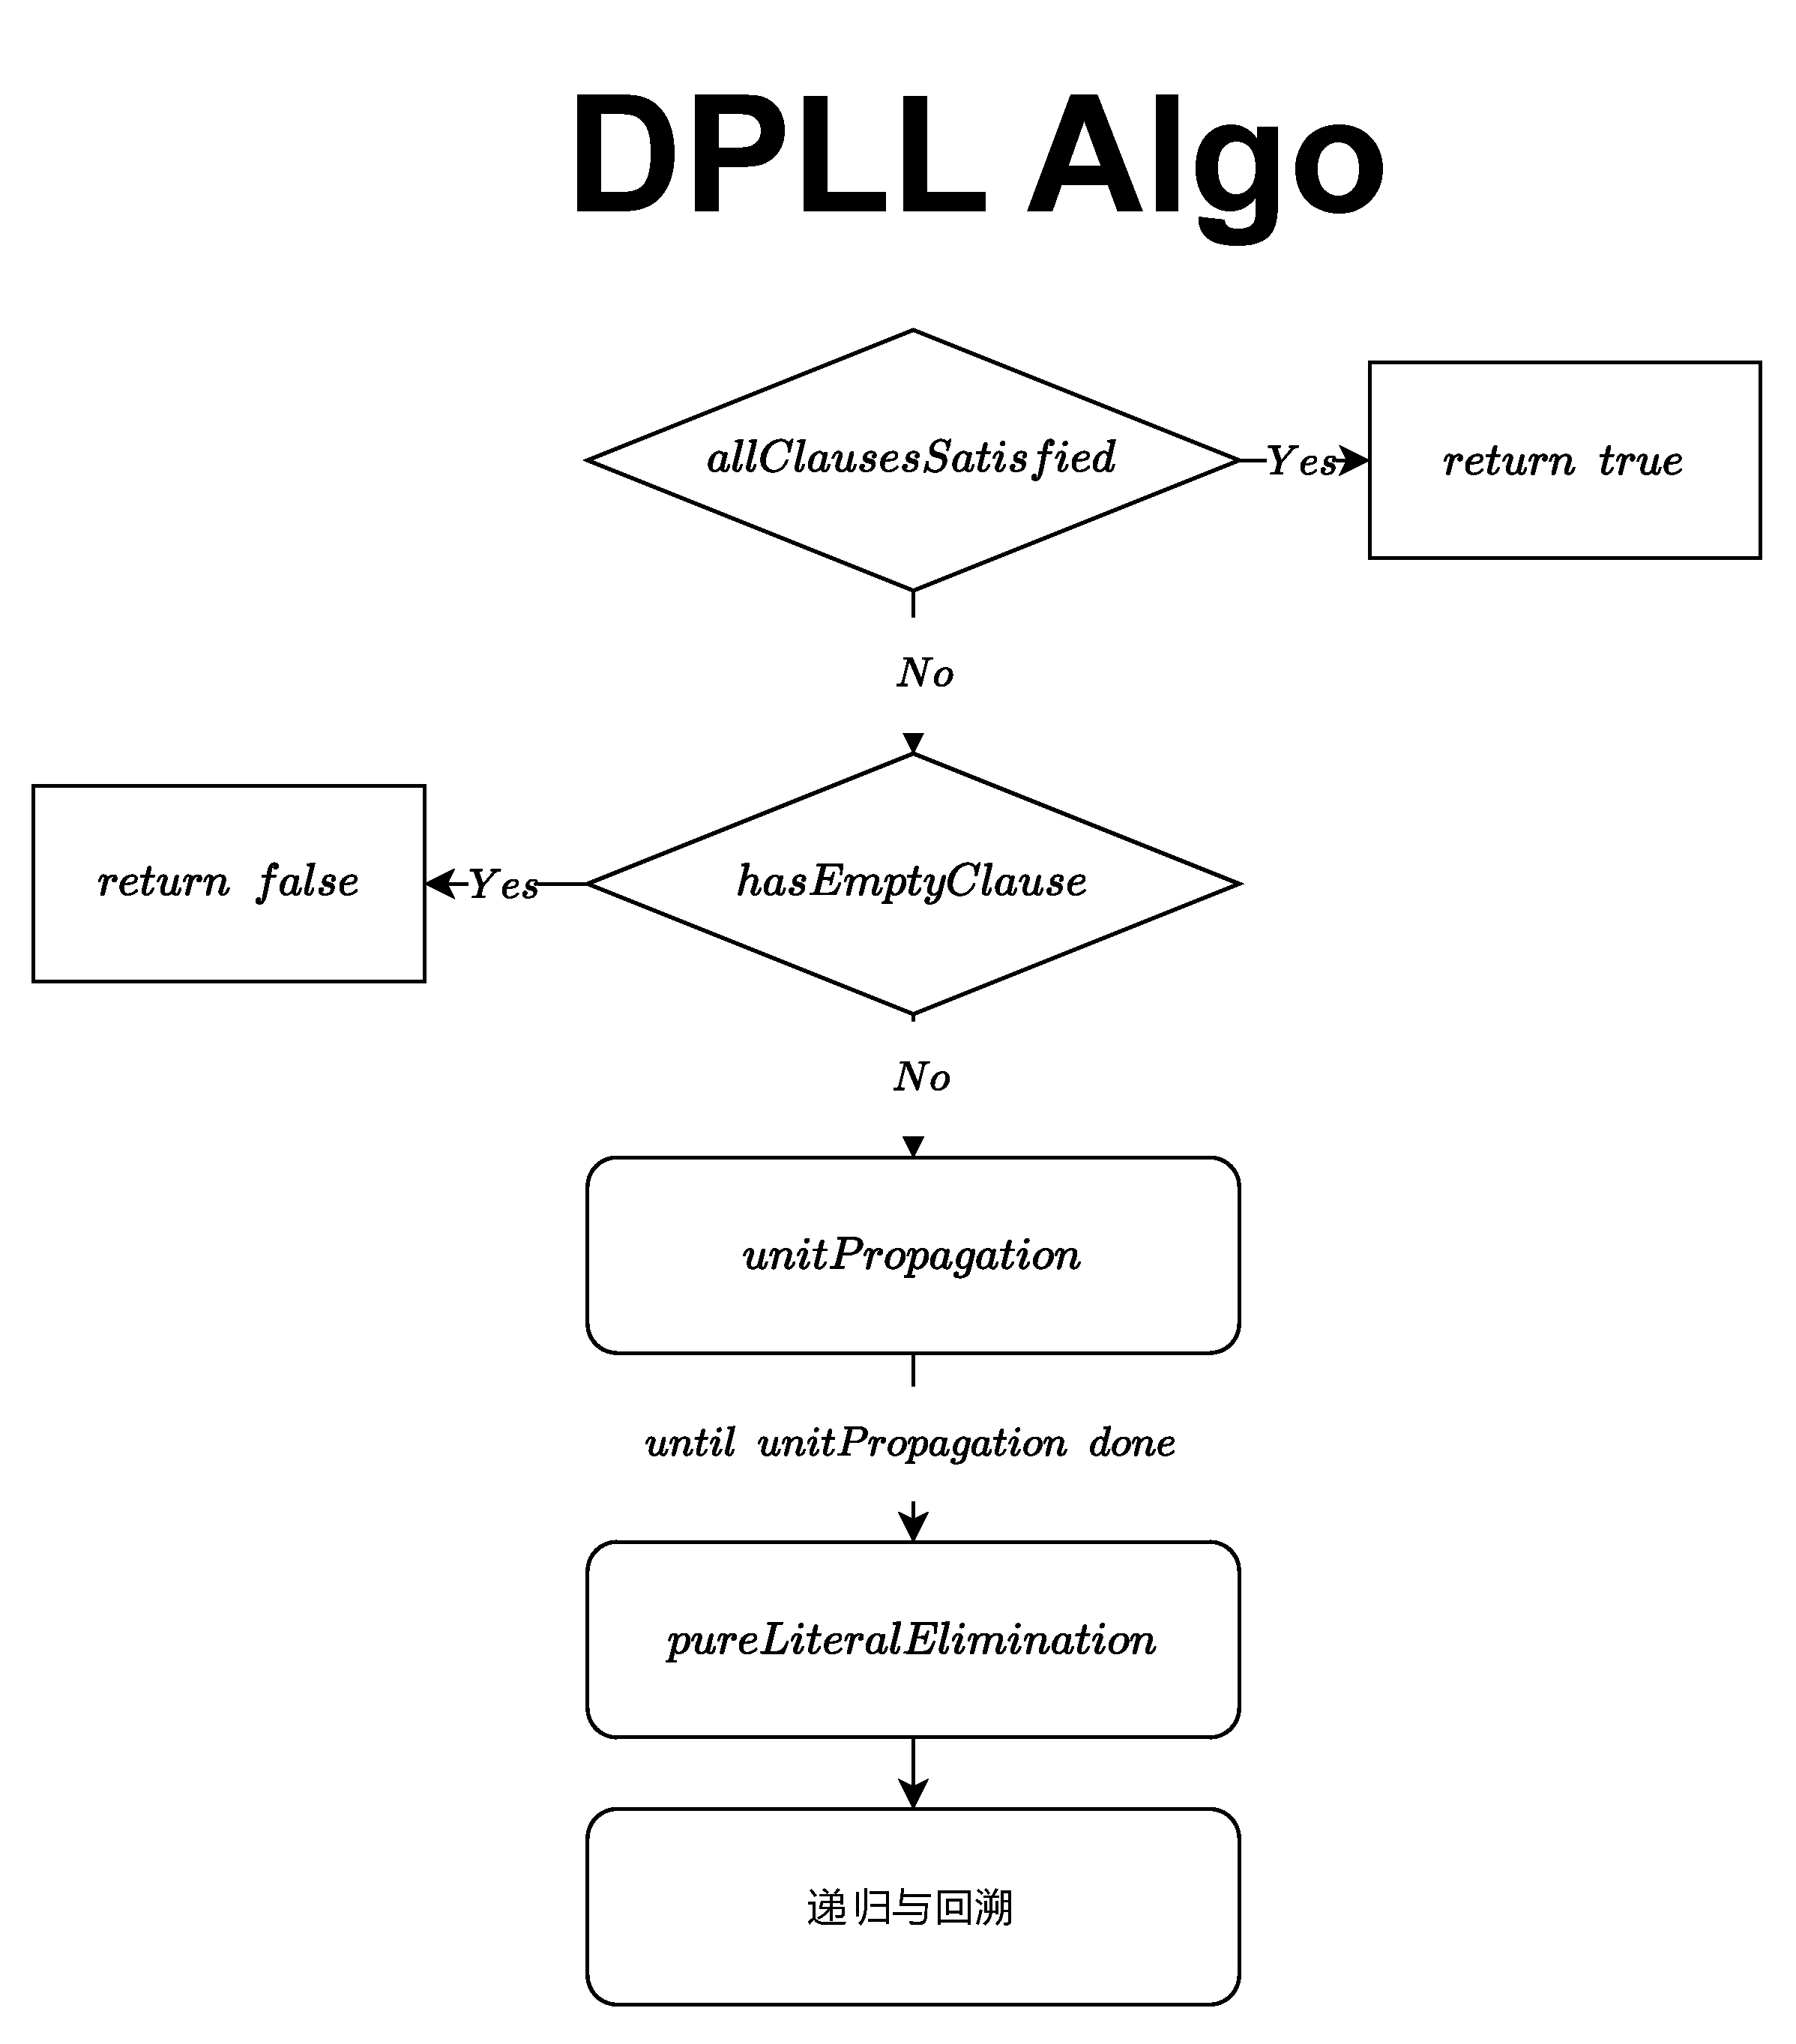
\includegraphics[width=10cm]{Figure/Figure_3.pdf}
            \caption{DPLL Algo}
        \end{figure}
        \noindent
        其实从这个流程图我们也可以看到:
        \par
        ``递归与回溯''这一步骤是在整个``DPLL算法''当中的最底部的,
        而``递归与回溯''是``回溯法''解决``SAT问题''的核心步骤,
        换言之,
        从本质上来讲,
        ``DPLL算法''就是``回溯法''
        \par
        而且从整个流程图当中,
        我们可以非常清晰地看到,
        我们在``递归与回溯''的上方加了几个预处理步骤
        \par
        至于``DPLL算法''中如何对处理``literal''方式的进行优化,
        我们会在``基于DPLL法的实现''中详细展开
        \subsubsection{WalkSAT算法}
            那么什么是``WalkSAT算法''呢?\par
            ``WalkSAT算法''是一种``非完备性算法'',
            本质上是对``贪心算法''的一种改进\par
            而我们主要基于``完备性算法''解决这个``3-SAT问题'',
            因此这里不展开讲``WalkSAT算法'',
            只是做一个简单的了解即可
\section{实现难点}
    \subsection{基于回溯法的实现}

        \subsubsection{当前子句可满足判断\ ——\ isCurrentClauseSatisfied}
        \noindent
        这个还是比较好理解的:\par
        (1)判断当前的``$clause_{i}$''的3个``$literal$''\par
        (2)如果存在某个``$literal_{j}$''的真值为true,
        即当前的这个``$clause_{i}$''的赋值为真,
        那么就return true,
        以此表示当前的这个``$clause_{i}$''是可满足的\\
        实现过程中也有几个\textbf{实现难点}:\par
        实现难点(1)如果获取``变量的编号''?\\
        我们先看一个例子:
        \begin{center}
            -2\ 5 \ 20
        \end{center}
        \noindent
        实际代表的意思是:
        \begin{center}
            $\overline{x_{2}} \cup x_{5} \cup x_{20}$
        \end{center}
        那么如何获取变量``$\overline{x_{2}}$''和``$x_{20}$''的编号呢?我这里进行了这么一个处理:
        \begin{lstlisting}
    int num_of_var = literal > 0 ? literal : -literal;
        \end{lstlisting}
        \noindent
        我们先考虑``$\overline{x_{2}}$'',注意到:
        \begin{center}
            $\overline{x_{2}}$在input过程中的$val=literal_{1}$是:\quad-2
        \end{center}
        那也就是说:
        \begin{center}
            我们只要对这个val取一个绝对值:\quad abs(-2)
        \end{center}
        这样我们就能获取``$\overline{x_{2}}$''的编号2\par
        同样地,我们考虑``$x_{20}$'',注意到:
        \begin{center}
            $x_{20}$在input过程中的$val=literal_{3}$是:\quad 20
        \end{center}
        类似地:
        \begin{center}
            我们也对这个val取一个绝对值:\quad abs(20)
        \end{center}
        这样我们就能获取``$x_{20}$''的编号20\par
        因此``获取变量的编号''就这么解决完毕了\\
        \newline
        当然了,实现过程中也有几个\textbf{实现细节}值得留意:\par
        实现细节(1)关于``获取`变量的编号' ''
        \begin{lstlisting}
        int num_of_var = literal > 0 ? literal : -literal;
        \end{lstlisting}
        \noindent
        实际上,我在``基于DPLL法的实现''改成了:
        \begin{lstlisting}
        int num_of_var = abs(literal);
        \end{lstlisting}
        这样改让这串代码的逻辑变得稍微清晰一点

        \subsubsection{布尔表达式可满足判断\ ——\ areAllClausesSatisfied}
        \noindent
        这个也比较好理解,而且思路也比较的常规:\par
        (1)通过遍历当前给定的布尔表达式中的
        m个``$clause$'',
        并且反复调用``$isCurrentClauseSatisfied$''函数,
        对每个``$clause$''单独进行判断,
        进而实现对给定的布尔表达式的判断。\par
        (2)只要存在某一个``$clause_{i}$''的真值为false,
        那也就相当于给定的布尔表达式是不可满足的,
        那么就return false,也就是说,
        给定的布尔表达式是不可满足的。\par
        由于整个实现过程中基本没有什么实现难点和实现细节需要留意,
        因此我们还是将整个讨论的重点放在:$\quad$``回溯法进行求解\ ——\ Solve\ ——\ 核心''上。
        
        \subsubsection{回溯法进行求解\ ——\ Solve\ ——\ 核心}
        \noindent
        首先,我们先指出实现过程中的几个\textbf{实现难点}:
        \par
        实现难点(1)如何对给定的布尔表达式中的n个变量进行$2^{n}$种bool assignment?
        (这是整个``回溯法''的核心)
        回答如下:
        \begin{center}
            利用\quad \underline{\textbf{递归赋值}}与\underline{\textbf{回溯}}\quad 进行bool assignment
        \end{center}
        \par
        那么具体上来讲,是如何实现这个过程的呢?我们来看看下面这串代码
        (``递归赋值''阶段)
        \begin{lstlisting}
            assignment[varIndex] = 1;
            if (Solve(varIndex + 1)){
                return true;
            }

            assignment[varIndex] = 0;
            if (Solve(varIndex + 1)){
                return true;
            }

            assignment[varIndex] = -1;
            return false;
        \end{lstlisting}
        这是什么意思呢?我们下面来解释一下:\par
        (1)先对$assignment[varIndex]$(我有一个专门的Part来进行解释)尝试bool assignment\par
        (2)通过$Solve(varIndex+1)$进入``递归赋值''与``回溯''阶段\\
        这个核心的``递归赋值''与``回溯''阶段是如何实现的呢?
        \par
        我们来看看下面这串代码
        \begin{lstlisting}
            assignment[varIndex] = 1;
            if (Solve(varIndex + 1)){
                ………………
            }
            ………………
        \end{lstlisting}
        \par
        最核心的实现逻辑就是:
        \begin{lstlisting}
            if (Solve(varIndex + 1))
        \end{lstlisting}
        \par
        将关注的点放在``Solve(varIndex+1)''上
        \newline
        \noindent
        我们可以知道:
        \par
        在完成了``assignment[varIndex]=1''后,
        我们进入到了``Solve(varIndex+1)''这个函数的内部
        \par
        再次观察一下这串代码:
        \begin{lstlisting}
            assignment[varIndex] = 1;
        \end{lstlisting}
        \par
        那么此时的``varIndex''就变成了``varIndex+1'',
        于是我们就对第$varIndex+1$个$literal$进行了bool assignment
        (当然我这里假设没有进入$areAllClausesSatisfied$函数当中,后面我们会看到)
        (后面有时间再改吧),
        因此实现了``递归赋值''的效果\par
        我们用一个最简单的布尔表达式
        (这个布尔表达式的子句就是布尔表达式本身),
        来演示一下这个过程,考虑:
        \begin{center}
            $\overline{x_{1}} \cup \overline{x_{2}} \cup \overline{x_{3}}$
        \end{center}
        \par
        首先$varIndex=1$,
        于是利用$assignment[varIndex=1]=1$,
        我们完成了这样一个bool assignment:
        \begin{center}
            $x_{1}=1$
        \end{center}
        \par
        然后我们会进入$Solve(varIndex+1=2)$这个函数的内部,
        同样地,利用$assignment[varIndex]=1$
        (需要注意的是:此时$varIndex=2$,
        并且同样没有进入到$areAllClausesSatisfied$函数当中),
        我们实现了这样一个bool assignment
        \begin{center}
            $x_{2}=1$
        \end{center}
        \par
        以此类推,最终这个布尔表达式将会被赋值为:
        \begin{center}
            $1 \cup 1 \cup 1$
        \end{center}
        \par
        然后我们会在solve(4)
        (因为$varIndex=3$的时候我们还没有进入到$if(varIndex > n)$的内部)
        中完成一个``$if(varIndex > n)$''判断,
        (至于为什么是这样,
        我们会在``回溯''阶段给出解释)
        \par
        观察下面的这串代码:
        \begin{lstlisting}
            if (varIndex > n) {
                if (areAllClausesSatisfied()) {
                    ………………
                    return true;
                }
                return false;
            }
        \end{lstlisting}
        接着,
        因为此时我们在Solve(4)中,
        因此$varIndex=4$,
        那么此时$varIndex=4>n=3$,
        于是,
        我们会进行$areAllClausesSatisfied$判断,
        我们会发现.
        给定的布尔表达式是不可满足的\par
        此时,我们会在``Solve(4)''中``return false''
        \par
        接着,观察下面的这串代码:
        \begin{lstlisting}
            assignment[varIndex] = 1;
            if (Solve(varIndex + 1)){
                return true;
            }
            assignment[varIndex] = 0;
            if (Solve(varIndex + 1)){
                return true;
            } 
        \end{lstlisting}
        \par
        那也就是说,
        我们跳出了if(Solve(varIndex+1)),
        下一步将会执行assignment[varIndex]=0
        (注意,此时的varIndex=3,
        因为我们已经从Solve(4)中跳回到Solve(3)当中了)
        \par
        因此,我们将会对``$x_{3}$''尝试一个新的bool assignment,
        即将``$x_{3}$''赋值为false,那么当前的这个``$clause$''就会转变为:
        \begin{center}
            $1 \cup 1 \cup 0$
        \end{center}
        \par
        同样地,我们会完成一个``$allClausesSatisfied$''判断
        (这里不再做解释了,
        主要还是因为我们步进到了$if(varIndex>n)$的内部进行$allClausesSatisfied$)\par
        如果此时整个布尔表达式已经是可满足的
        (就这个例子而言这个布尔表达式已经是可满足的),
        我们将会在Solve(varIndex+1)中return true
        观察下面这串代码:
        \begin{lstlisting}
            assignment[varIndex] = 1;
            if (Solve(varIndex + 1)){
                return true;
            }
            assignment[varIndex] = 0;
            if (Solve(varIndex + 1)){
                return true;
            } 
        \end{lstlisting}
        \par
        因为我们已经在Solve(varIndex+1)中return true,
        也就是说,
        我们下一步将会执行if(Solve(varIndex+1))内的语句,
        也就是return true
        \par
        就此刻而言,
        我们已经求解成功了,
        因为我们已经在Solve这个函数中return true,
        表示当前这个布尔表达式是有可行解的
        \par
        很自然地,下一步我们将会执行cout bool assignment这一阶段,
        我们看下面这一串代码就可以很清晰地知道了(其他具体细节就不一一展示了):
        \begin{lstlisting}
            ………………
            for (int i = 1; i <= n; i++) {
                cout << assignment[i];
                if (i != n){
                    cout << " ";
                } 
            }
            cout << endl;
            ………………
        \end{lstlisting}
        \par
        如果此时整个布尔表达式还是不可满足的
        (当然这个例子中该布尔表达式已经是可满足的,
        但为了更好地进行解释,
        我们一并进行解释)
        \par

        首先,我们来重新看一下目前这个布尔表达式的赋值:
        \begin{center}
            $1\quad 1 \quad 0$
        \end{center}
        \par
        还是观察下面的这串代码:
        \begin{lstlisting}
            if (varIndex > n) {
                if (areAllClausesSatisfied()) {
                    ………………
                    return true;
                }
                return false;
            }
        \end{lstlisting}
        \par
        因为这个布尔表达式是不可满足的,
        那也就是说,
        我们并不会进入到$if(allClausesSatisfied)$的内部,
        因此下一步我们将会return false
        (注意,
        我们是在Solve(4)中return false,
        至于为什么,
        可以重新再看一下if(varIndex>n))

        \par

        接着,我们观察一下这么一串代码:

        \begin{lstlisting}
            assignment[varIndex] = 1;
            if (Solve(varIndex + 1)){
                return true;
            }
            assignment[varIndex] = 0;
            if (Solve(varIndex + 1)){
                return true;
            } 
            assignment[varIndex] = -1;
            return false;
        \end{lstlisting}
        \par
        因为我们在Solve(varIndex+1)中return false,
        那也就是说,
        下一步我们将会执行assignment[varIndex]=1这一步,
        也就是说,我们将会把$x_{3}$赋值为-1
        (关键的``回溯''阶段),
        那么整个布尔表达式就变成了:
        \begin{center}
            $1 \cup  1 \cup -1$
        \end{center}
        
        \par
        再下一步,
        很明显,
        我们将会执行return false,
        也就是说,
        我们将会在Solve(3)中return false,
        此时,
        我们将会回到Solve(2)当中
        \par
        同样,观察下面这串代码:
        \begin{lstlisting}
            assignment[varIndex] = 1;
            if (Solve(varIndex + 1)){
                return true;
            }
            assignment[varIndex] = 0;
            if (Solve(varIndex + 1)){
                return true;
            }
        \end{lstlisting}
        \par
        由于此时的``varIndex''是`2',
        那也就是说,
        下一步我们将会从if(Solve(varIndex+1))中跳出,
        执行assignment[varIndex]=0,
        也就是说,
        我们将对``$x_{2}$''尝试新的bool赋值,
        即我们会将``$x_{2}$''赋值为0,
        那么此时的这串``$clause$''就变为:
        \begin{center}
            $1 \cup 0 \cup -1$
        \end{center}
        \par
        此时,观察下面的这串代码:
        \begin{lstlisting}
            assignment[varIndex] = 0;
            if (Solve(varIndex + 1)){
                return true;
            }
        \end{lstlisting}
        \par
        我们会发现,
        我们重新进入到了Solve(varIndex+1)当中开始新一轮的赋值,
        我这里直接给出结果:
        \begin{center}
            $1 \cup 0 \cup 1$
        \end{center}
        \begin{center}
            $1 \cup 0 \cup 0$
        \end{center}
        \begin{center}
            $\vdots$
        \end{center}
        \par
        由此往复,
        我们会不断尝试新的bool赋值,
        直到给定的布尔表达式有解为止
        (当然也可能没有解,
        不过这个可能性还是非常非常小的,
        因此我们主要考虑更可能出现的情况
        \ ——\ 
        布尔表达式是可满足的)
        \par
        在这么一个循环的结构下,
        我们实现了对``$clause$''当中的n个变量进行$2^{n}$种bool赋值,
        以此来求出给定的布尔表达式的可行解
        (实际上可能不用进行这么多次判断,
        但这已经是最差的情况了,
        因为在这种情况下每种assignment都经过了``$areAllClausesSatisfied$''判断,
        即我们对给定的布尔表达式的每种可能的assignment都进行了判断)
        \par
        这就是整个``回溯法''中
        最核心的
        ``\underline{\textbf{递归赋值}}''
        与
        ``\underline{\textbf{回溯}}''
        阶段。
        \newline
        \par
        实现难点(2)如果我成功进行了bool赋值,
        那么如何合理地编排各个函数的顺序判断给定的布尔表达式是可满足的呢?
        \newline
        \par
        其实从上面的分析我们已经对整个``回溯法''的实现过程有一个比较清晰的了解了,
        不过这里我们还是来简单地分析一下代码实现的logic,
        首先我们先观察一下整串代码
        (我这里把注释全都删掉了,当然我也有备份处理):
        \begin{lstlisting}
        bool Solve(int varIndex) {
            if (varIndex > n) {
                if (allClausesSatisfied()) {
                    for (int i = 1; i <= n; i++) {
                        cout << assignment[i];
                        if (i != n){
                            cout << " ";  
                        } 
                    }
                cout << endl;
                return true;
                }
            return false;
            }
            递归赋值 与 回溯
        }
        \end{lstlisting}
        我们从两个``Part''来进行说明:\par
        Part(1)什么时候开始对给定的布尔表达式进行判断?\par
        Part(2)什么时候进行``递归赋值与回溯''?\\
        我们先来看看``Part(1)'':
        $\quad$``什么时候对给定的布尔表达式进行判断''?
        \begin{lstlisting}
        if ( varIndex > n){
            ………………
        }
        \end{lstlisting}
        \par
        从代码上进行解释,
        只有当``$clause$''中的所有``$literal$''都已经完成赋值的时候,
        我们才开始对每个``$clause$''
        (当然也可以说是单个``$clause$''),
        即对给定的布尔表达式进行判断\par
        \begin{lstlisting}
        if (areAllClausesSatisfied()) {
            ………………
        }
        \end{lstlisting}
        \par
        很自然地,当给定的布尔表达式是可满足的时候,我们输出assignment的结果
        (具体实现看代码即可):
        \begin{lstlisting}
                ………………
                cout << assignment[i];
                if (i != n){
                cout << " ";  
                } 
                ………………
        \end{lstlisting}
        \par
        我们再来看看``Part(2)'':$\quad$``什么时候进行`递归赋值'与`回溯'\ ''?
        \par
        我们先观察一下下面这串代码:
        \begin{lstlisting}
            if (varIndex > n) {
                ………………
            }
            assignment[varIndex] = 1;
            ………………
            assignment[varIndex] = 0;
            ………………
            assignment[varIndex] = -1;
            ………………
        \end{lstlisting}
        \par
        很自然地,
        当然是当前的这个``$clause$''的所有``$literal$''都还没有进行了bool assignment
        (因为我们始终都没有进入到if(varIndex>n)的内部),
        我们进行``递归赋值''(具体看(1)中的解释)
        \par
        至于``回溯''阶段,
        我们从上面的分析也可以知道,
        只要当前的这个bool assignment不能使给定的布尔表达式是可满足的,
        我们就不断尝试新的bool assignment,
        不断地判断给定的布尔表达式是否是可满足的,
        不断地进行``回溯'',
        直到给定的布尔表达式是可满足的为止
        至此,
        对于整个``回溯法''的处理过程,
        我们现在已经有了一个清晰的认知。
        \subsubsection{实现过程中的小细节}
        \noindent
        \textbf{实现细节}(1)$\quad$
        ``isCurrentClauseSatisfied''函数
        当中的
        ``\underline{引用}''
        与
        ``赋值''
        \begin{lstlisting}
        Clauses& clause = AllClauses[clauseIndex];
        \end{lstlisting}
        \par
        我这里进行了这么一个处理:
        \begin{lstlisting}
        Clauses : "引用"处理
        \end{lstlisting}
        \par
        那我为什么要这么做呢?实际上,一开始我是按照下面这么干的:
        \begin{lstlisting}
        Clause clause = AllClauses[clauseIndex];
        \end{lstlisting}
        \par
        虽然通过``赋值''进行处理
        (我重构了代码,所以实际上的代码可能看起来不像``赋值''处理)也是OK的
        (当然实现过程中也出现了许多奇奇怪怪的bug),
        但后面进行优化的时候发现使用``引用''可以避免不必要的内存开销。
    \subsection{基于DPLL法的实现}

        \subsubsection{当前子句可满足判断\ ——\ isCurrentClauseSatisfied}
            从本质上来讲,
            实现的思路与``回溯法''中的``当前子句判断\ ——\ isCurrentClauseSatisfied''是一样的,这里不做过多叙述
        \subsubsection{布尔表达式可满足判断\ ——\ areAllClausesSatisfied}
            同样地,实现的思路与``回溯法''中的``布尔表达式可满足判断
            \ ——\ areAllClausesSatisfied''是一样的
            (实际上是一模一样的,
            因为我直接copy paste过去了),
            这里也不做过多叙述
        \subsubsection{空子句判断\ ——\ hasEmptyClause\ ——\ 核心}
        \noindent
        在``解题方法简介''当中,我们已经指出:
        \par
            ``DPLL算法''的本质就是在执行``回溯法''之前对``$literal$''进行各种预处理操作
        \\
        \noindent
        \newline
            那么``空子句判断''是如何对``$clause$''中的``$literal$''进行预处理的呢?
        \\
        \noindent
        \newline
        我们从下面几个问题来对此进行分析:\\
            \par
            (1)什么是``空子句判断\ ——\ hasEmptyClause''?\par
            (2)为什么要进行``空子句判断''?\par
            (3)怎么实现``空子句判断''?\\
        \newline
        我们先来回答(1):   ``什么是空子句?''\\
        \par
        同样地,我们拿一个简单的例子来进行说明,考虑:
        \begin{center}
            $clause_{1} = x_{1} \cup x_{2} \cup x_{3}$
        \end{center}
        \begin{center}
            $clause_{2} = \overline{x_{1}} \cup \overline{x_{2}} \cup \overline{x_{3}}$
        \end{center}
        \begin{center}
            $clause_{3} = \overline{x_{1}} \cup x_{2} \cup \overline{x_{3}}$
        \end{center}
        \par
        我们现在考虑这么一个assignment:
        \begin{center}
            $x_{1}=x_{2}=x_{3}=true$
        \end{center}
        \par
        那么,我们可以非常清晰地看到这么一个事实:
        \begin{center}
            $clause_{1}:true$
        \end{center}
        \begin{center}
            $clause_{2}:false$
        \end{center}
        \begin{center}
            $clause_{3}:true$
        \end{center}
        \par
        那也就是说:
        \begin{center}
            $clause_{2}$是一个空子句
        \end{center}
        \par
        我们这里直接指出``空子句''的定义:\\
        if$\ \exists$ 一组bool assignment 
        S.t. $clause_{j}$ 的真值为 false,那么该$clause_{j}$就是一个空子句。
        \newline
        \par
        那么我们现在来回答(2):   ``为什么要进行空子句判断?''\\
        \par
        同样,我们还是考虑上面的例子:
        \begin{center}
            $clause_{1} = x_{1} \cup x_{2} \cup x_{3}$
        \end{center}
        \begin{center}
            $clause_{2} = \overline{x_{1}} \cup \overline{x_{2}} \cup \overline{x_{3}}$
        \end{center}
        \begin{center}
            $clause_{3} = \overline{x_{1}} \cup x_{2} \cup \overline{x_{3}}$
        \end{center}
        \par
        我们也考虑同样的assignment:
        \begin{center}
            $x_{1}=x_{2}=x_{3}=true$
        \end{center}
        \par
        我们来观察这么一个事实,考虑:
        \begin{center}
            $clause_{2}=false$
        \end{center}
        \begin{center}
            $clause_{3}=true$
        \end{center}
        \par
        很明显,
        ``$clause_{2}$''是一个``空子句'',
        因为当的这个``$clause_{2}$''的真值为false
        \par
        很自然地,就有这么一个问题:
        \begin{center}
            我们对``$clause_{3}$''$(clause_{4},\cdots,\cdots,)$进行其他赋值还有意义吗?
        \end{center}
        \par
        非常可惜的是,这么做并没有什么意义。
        \par
        也就是说,只要给定的布尔表达式中存在``空子句'',
        我们就不用对``空子句''
        (在这个例子当中是``$clause_{2}$'')
        后面的``$clause$''(此处是``$clause_{3}$'')进行判断。
        \par
        那么,很自然地,我们会问这么一个问题:
        \begin{center}
            我们应该如何进行处理呢?    
        \end{center}
        \par
        我们只需在当前的这个``空子句''进行``\textbf{回溯}''
        (要么就是递归赋值,要么就是回溯并递归赋值,后面有时间再改改)''操作,
        重新对``$clause_{2}$''尝试其他的bool assignment即可,
        然后接着进行``\textbf{递归赋值}''操作,
        对``$clause_{3}$''进行bool assignment即可,
        这样可以非常有效地降低复杂度,
        提高整个算法的运行效率。
        \par
        这么看来,``判断空子句''还是非常的有必要的。
        \newline
        \par
        现在我们来回答(3):$\quad$``如何实现空子句判断''?
        \newline
        \par
        在实现``空子句判断''的过程中,也存在着这么几个\textbf{实现难点}:\\
        \par
            (3.1)如何判断当前的这个``$clause_{i}$''是不是``空子句''?\par
            (3.2)如果当前的这个``$clause_{i}$''是``空子句'',我们做什么样的处理呢?
        \newline
        \par
        我们先来回答(3.1):$\quad$ ``怎样判断当前的这个`$clause_{i}$'是一个空子句''
        \newline
        \par
        那么,到底怎么来判断当前的这个``$clause_{i}$''是一个``空子句''呢?
        \par
        十分自然地,
        从定义上来看,
        只需要当前的这个``$clause_{i}$''的3个``$literal$''都不能使得``$clause_{i}$''的赋值为真即可,
        此时我们可以说当前的这个``$clause_{i}$''是一个``空子句''
        \par
        具体来讲,我们看一下下面这串代码:
        \begin{lstlisting}
                if (allLiteralFalse) {
                    return true;
                }
        \end{lstlisting}
        \par
        从代码上进行解释,
        如果当前的这个``$clause_{i}$''是一个空子句,
        也就是说,
        对``$clause_{i}$''中的所有``$literal$''的bool assignment
        都不能使得``$clause_{i}$''的赋值为真,
        因此,
        很自然地,
        $allLiteralFalse$也就是true了,
        也就是说,
        我们下一步将会return true,
        表示给定的布尔表达式中含有空子句,
        并且这个空子句就是``$clause_{i}$''
        \par
        很自然地,针对当前的这个``$clause_{i}$''不是一个``空子句'', 
        即存在某个``$literal$''使得当前的这个``$clause_{i}$''的赋值为真,
        我们会有这么一个问题:
        \par
        如果我们已经找到了某个``$literal_{j}$'' 
        S.t. 当前的这个``$clause_{i}$''的真值为真,
        那我们还需要对下一个``$literal_{j+1}$''进行判断吗?
        \par
        很明显,根本不用!因为我们已经让当前的这个``$clause_{i}$''的赋值为真,
        我们只需要对``$clause_{i+1}$''进行同样的判断就可以了,
        我们这里看一下这串代码:
        \begin{lstlisting}
        if ( ……条件稍微长了一点……) {
            allLiteralFalse = false;
            break;
        }
        \end{lstlisting}
        \par
        实际上就是说,
        只要我在遍历``$clause_{i}$''中的每个``$literal$''过程中,
        发现某个``$literal_{j}$''使得``$clause_{i}$''的真值为true,
        我们就设定$allLiteralFalse$为false,
        也就是说,
        我们认为当前的这个``$clause_{i}$''不是一个空子句,
        因此,
        我们直接break出for loop对下一个``$clause_{i+1}$''进行新一轮的判断即可
        \par
        但是我们需要解决这么一个问题:
        \par
        根据上面的判断方式,
        我们默认当前的这个``$clause_{i}$''中的每个``$literal$''都已经赋值了,
        但是如果有某个``$literal_{j}$''还未进行赋值的话,我们应该怎样进行处理呢?
        \par
        我们来看看下面这串代码:
        \begin{lstlisting}
            if (assignment[var] == -1) {
                allLiteralFalse = false;
                break;
            }
        \end{lstlisting}
        \par
        我们可以很清楚地看到,
        我们将``$allLiteralFalse$''设为了false,
        也就是说,
        我们认为当前的这个``$clause_{i}$''不是一个空子句
        (毕竟非空子句出现的可能多一点,
        只需要$clause$中的某个$literal$使得整个$clause$的真值为true即可)
        \par
        因此,
        很自然地,
        我们只需要break出for loop,
        对下一个``$clause_{i+1}$''进行同样的判断即可
        \newline
        \par
        我们现在来回答(3.2):
        $\quad$``在判断`$clause_{i}$'不是一个空子句后,
        我们下一步应该如何进行处理''?
        \newline
        \par
        很显然,
        我们只需要对下一个``$clause_{i+1}$''进行同样的判断
        (我这里省略掉了中间break的实现过程)
        即可,
        具体看下面这串代码即可:
        \begin{lstlisting}
        bool hasEmptyClause() {
            for (int i = 0; i < m; i++) {
                ……………………
            }
            return false;
        }
        \end{lstlisting}
        \par
        那也就是说,
        我们最终会将整个布尔表达式的所有``$clause$''都进行一次判断,
        看看能不能从中找出空子句,
        如果找出了空子句,
        我们会认为给定的布尔表达式是没有可行解的
        (后面在DPLL我们会解释为什么这样子),
        如果没有找出空子句,
        我们将会进行下一个阶段\ ——\ ``单位子句传播''
        \par
        至此,我们已经将``怎样判断空子句''叙述清楚了。
        
        \subsubsection{单位子句传播\ ——\ unitPropagation\ ——\ 核心}
        ``单位子句传播''是如何对``$clause$''中的``$literal$''进行预处理的呢?
        \\
        \noindent
        \newline
        同样地,我们也以这么几个问题进行展开:\\
            \par
            (1)什么是``单位子句传播\ ——\ unitPropagation''?\par
            (2)为什么要进行``单位子句传播''?\par
            (3)怎么实现``单位子句传播''?\\
        \noindent
        \newline
        同样,我们先来回答(1):   ``什么是单位子句传播?''\\
        \par
        同样地,我们拿一个简单的例子来进行说明,考虑:
        \begin{center}
            $clause_{1} = x_{1} \cup x_{2} \cup \overline{x_{3}}$
        \end{center}
        \par
        我们这里令:
        \begin{center}
            $x_{1}=x_{2}=false$
        \end{center}
        \par
        也是十分明显地,我们必须将``$x_{3}$''赋值为false,
        才能使得这个``$clause_{1}$''的赋值为真,
        否则的话,
        这个``$clause_{1}$''就是一个空子句了
        \par
        我们这里指出,这里的这个``$clause_{1}$''就是一个``单位子句''
        \par
        很自然地,我们会问:``单位子句''的定义是什么呢?
        \par
        我们这里给出``单位子句''的定义:
        \par
        子句``$clause$''中\underline{有且仅有一个未赋值}的``$literal$''就是一个``单位子句''
        \par
        也就是说,
        我们在``$clause$''不为空子句的情况
        (当然此时还满足某些特殊的条件,
        我们下面再展开叙述)下,
        做了某些特定的操作
        (其实这个操作就是``单位子句传播''的过程)。
        \par
        此时,
        我们固定这个``$x_{3}$''的赋值(``$x_{3}$''已经赋值为false)
        \par
        也就是说,我们固定``$assignment[3]$''的赋值也为false
        \\
        这么处理的话,
        我们只需要对布尔表达式中剩余的``$clause$''中的那些变量
        (注意,这里是变量,不是``$literal$'')
        进行bool assignment即可
        \par
        也就是说,
        通过对特定的``非空子句''进行判断,
        我们可以将某个``$literal$''的bool assignment传播到整个布尔表达式
        \par
        这就是``单位子句传播''的过程。
        \newline
        \par
        \noindent
        我们现在来回答(2):   ``为什么要进行单位子句传播''
        \newline
        \par
        其实通过比对``回溯法''和上面的这个例子我们可以看出:
        通过进行``单位子句传播'',
        我们可以极大地提升整个算法的运行效率\par
        为什么这么说呢?
         我们已经在``基于回溯法的实现''中看到,
        ``回溯法''的本质就是``不成功就推倒重来''
        \ ——\ 
        虽然没有什么毛病,
        但毫无疑问的是,
        这么做运行时间会变得非常非常长,
        因为布尔表达式中每个变量都有2种出现的方式:
        $pos\ literal$和$neg\ literal$,
        因此实际的复杂度可能是$o(2^{n})$(我还有点不确定),
        当然有可能更加的久,
        但可以肯定的一点是,
        这个求解时间一定是非常非常长的,
        尤其是遇到数据量比较大的测例,
        之前也吐槽过这一点。
        \par
        而在上面的这个例子中,
        我们选择了固定``$literal$''的bool assignment,
        并将它传播到整个布尔表达式当中,
        毫无疑问,
        省去了``推倒重来''这么一个过程,
        可以极大地提高算法的运行效率。
        \par
        因此,同样地,进行``单位子句传播''也是一件非常有必要的事。\\
        \newline
        \noindent
        最后,我们现在来回答(3):   ``怎么进行单位子句传播''
        \newline
        \par
        同样,在实现``单位子句传播''的过程中,也存在着这么几个\textbf{实现难点}:
        \newline
        \par
            (3.1)如何判断当前的这个``$clause_{i}$''是不是``单位子句''?\par
            (3.2)如果判断当前的这个``$clause_{i}$''是``单位子句'',那如何进行``单位子句传播''呢?\\
        \par
        我们来回答一下(3.1):$\quad$``如何判断当前的这个`$clause_{i}$'是不是单位子句''?
        \\

        首先,我们来看一下这串代码(我在这里保留原始的注释):
        \begin{lstlisting}
        // 初始化用于记录"clause中未进行bool赋值的literal个数" 
        int unassignedLiteralCounter = 0;
        // 初始化用于记录"当前clause中最后一个未赋值的literal"
        int lastUnassignedliteral = 0;
        // 初始化用于记录"S.t.当前clause satisfied的literal"
        int satisfiedLiteral = 0;
        \end{lstlisting}
        \par
        很自然地,根据``单位子句''的定义:
        子句``$clause$''中\underline{有且仅有一个未赋值}的``$literal$''是一个``单位子句'',
        我们可以知道下面这两点
        \par
        (1)当前``$clause_{i}$''中未赋值的$literal$''的个数为1,
        也就是说,
        $unassignedLiteralCounter=1$
        \par
        (2)当前``$clause_{i}$''还是不可满足的
        (若非,我会在代码中直接break出loop判断下一个``$clause_{i+1}$''),
        即使得当前的``$clause_{i}$''为可满足的``$literal$''个数为0,
        也就是说,
        $satisfiedLiteral=0$
        (实际代码中的意义并非如此,
        只不过我这里就这么说了,
        其实这么看来好像也没有什么毛病)
        \par
        因此会有下面的这么一串代码:
        \begin{lstlisting}
        if (
            unassignedLiteralCounter == 1 
            && 
            satisfiedLiteral == 0
            ) {
                ………………
                propagated = true;
        }
        \end{lstlisting}
        \par
        那也就是说,
        只要满足了上面的条件
        (可能条件还定义的不够严谨)
        我们就可以判断出当前的这个``$clause_{i}$''是一个单位子句,
        需要进行相关的处理。
        \newline
        \newline
        其中:
        \par
        这里的``propagated = true''
        表示当前的这个``$clause_{i}$''需要进行``单位子句传播''处理(后面会再进行说明)
        \newline
        \par
        现在我们来回答一下(3.2):
        $\quad$ 在成功判断当前``$clause_{i}$''是单位子句的基础上,
        ``如何实现`单位子句传播''?
        \newline
        \par
        我们这里先给出代码实现的核心部分,代码如下:
        \begin{lstlisting}
    bool unitPropagation() {
        bool propagated = false;
        for (int i = 0; i < m; i++) {
            ………………
            for (int j = 0; j < 3; j++) {
                ………………
                if (assignment[num_of_var] == -1) {  
                    unassignedLiteralCounter++;
                    lastUnassignedliteral = literal;
                } 
                else if ((满足条件(跟之前的条件类似))) {
                    satisfiedLiteral = literal;  
                }
            }
            if (unassignedLiteralCounter == 1 && satisfiedLiteral == 0) {
                int num_of_var = abs(lastUnassignedliteral);
                assignment[num_of_var] = (lastUnassignedliteral > 0) ? 1 : 0;
                propagated = true;
            }
        }
        return propagated;
    }
        \end{lstlisting}
        \par
        现在我们来分析一下这串代码的实现逻辑,首先我们看一下下面这个segment:
        \begin{lstlisting}
        if (assignment[num_of_var] == -1) {  
            unassignedLiteralCounter++;
            lastUnassignedliteral = literal;
        } 
        \end{lstlisting}
        \par
        很自然地,
        我们会对``$clause_{i}$''中的每个``$literal$''进行遍历,
        因为我们的目标是找出当前的这个``$clause_{i}$''
        中还没有进行bool assignment的``$literal_{j}$'',
        因此,
        只要``$literal_{j}$''还没有进行赋值,
        也就是说,
        $assignment[num\_of\_var]=-1$,
        我们就会让``$unassignedLiteralCounter$''这个计时器+1,
        并且,
        我们会将当前的这个``$literal_{j}$''记录到``$lastUnassignedliteral$''当中(为了下一步判断)。
        \par
        我们现在来看下面这串代码:
        \begin{lstlisting}
        if (unassignedLiteralCounter == 1 && satisfiedLiteral == 0) {
        int num_of_var = abs(lastUnassignedliteral);
        assignment[num_of_var] = (lastUnassignedliteral > 0) ? 1 : 0;
        propagated = true;
        }
        \end{lstlisting}
        \par
        我们先观察这个条件
        ``unassignedLiteralCounter == 1 \&\& satisfiedLiteral == 0'',
        也就是说,我们认为当前的这个``$clause_{i}$''是需要进行``单位子句传播''的,
        因此我们完成了两个操作:
        \par
        (1)将$assignment[num\_of\_var]$
            按照该变量在``$clause_{i}$''中出现的方式
            (``$pos \ literal$''或``$neg \ literal$'')
            进行bool assignment
        \par
        (2)将``$bool\ propagated$''赋值为``true'',
            表示当前的这个``$clause_{i}$''是需要进行``单位子句传播''的,
            也就是说,
            我们在这个function内做了``单位子句传播''这么一个操作,
            这相当于一个记号,
            因为在DPLL Algo内我们会不断地触发``单位子句传播''这么一个过程
            (我只需要将这整个function放置在一个while loop内,
            让这个function不断返回true,
            直到返回false,
            也就是不用再进行单位子句传播即可)

        \par
        很自然地,
        在上面的这个讨论中,
        会有这么一个问题:
        我们所有的讨论都是基于当前的这个``$clause_{i}$''
        存在``$literal_{j}$''未进行bool assignment
        \par
        那如果说:
        当前的这个``$clause_{i}$''中的
        每个``$literal$''都进行了bool assignment呢?我们会怎么进行处理呢?
        \par
        我们还是来看下面这一串代码:
        \begin{lstlisting}
        else if (满足条件) {
            satisfiedLiteral = literal;  
        }
        \end{lstlisting}
        \par
        我这里做了这么一个处理:
        我将每个已经完成了bool assignment的``$literal$''放进了``$satisfiedLiteral$'',
        也就是说,
        我只是做了一个纯粹的``记录''工作,
        当然,
        我在``判断单位子句''的过程中也很巧妙地运用了这个点
        \par
        我们来看下面一串代码:
        \begin{lstlisting}
        if (……………… && satisfiedLiteral == 0) {
        ………………
    }
        \end{lstlisting}
        \par
        我们看一下``$satisfiedLiteral == 0$''这个操作,
        可以从input``$literal$''的过程中很清楚地知道:
        ``$satisfiedLiteral$''要么等于0,要么不等于0
        \par
        只要$literal_{j}$使得$clause_{i}$的赋值为真,
        那么就将$literal_{j}$赋值给$satisfiedLiteral$,
        此时的这个$satisfiedLiteral$一定不为0,
        因为$literal_{j}$本身就不可能为0(总不能有$x_{0}$吧)
        \par
        如果所有的$literal$都不能使得$clause_{i}$的赋值为真,
        那也就是说,
        此时根本就没有将$literal_{j}$赋值给$satisfiedLiteral$这个过程,
        因为之前已经将$satisfiedLiteral$初始化为0,
        那也就很自然地满足$satisfiedLiteral==0$这个条件,
        因而就会进入到$if(\cdots \&\& satisfiedLiteral ==0)$这个条件语句的内部了
        \par
        其实在写整个function的过程有几个比较有意思的点,先看一下下面这串代码:
        \begin{lstlisting}
        for (int j = 0; j < 3; j++) {
        ………………
        if (assignment[num_of_var] == -1) {  
            ………………
        } 
        else if (………………) {
            ………………
        }
    }
        \end{lstlisting}
        \par
        可以看到这串代码当中是没有最后的``else''的,为什么这么做呢?
        主要还是因为整个function的目标是找出``$clause_{i}$''中
        最后一个未进行bool assignment的``$literal$'',
        换言之,
        我只关心``最后一个$literal$'',
        至于说``$literal$''已经进行了bool assignment
        但是``$clause_{i}$''是不可满足的
        (我这里指出一下前两个条件:
        未进行bool assignment的;
        进行了bool assignment并且满足条件的),
        这不是我们需要focus的点。
        \par
        就目前而言,
        我们已经对``单位子句传播''的过程有了一个非常清晰的认识了。
        
        \subsubsection{孤立文字消去\ ——\ pureLiteralElimination\ ——\ 核心}
        \noindent
        同样地,
        ``孤立文字消去''是如何对``clause''中的``literal''进行预处理的呢?
        \\
        \noindent
        \newline
        \noindent
        同样地,我们也以这么几个问题进行展开:\\
            \par
            (1)什么是``孤立文字消去\ ——\ pureLiteralElimination''?\par
            (2)为什么要进行``孤立文字消去''?\par
            (3)怎么实现``孤立文字消去''?\\
        \noindent
        \newline
        同样,我们先来回答(1):   ``什么是孤立文字消去?''\\
        \par
        同样地,我们拿一个简单的例子来进行说明,考虑:
        \begin{center}
            $clause_{1} = x_{1} \cup \overline{x_{2}} \cup x_{3}$
        \end{center}
        \begin{center}
            $clause_{2} = x_{1} \cup x_{2} \cup x_{3}$
        \end{center}
        \begin{center}
            $clause_{3} = x_{1} \cup x_{2} \cup \overline{x_{3}}$
        \end{center}
        \par
        我们会注意到这么一个事实:
        \begin{center}
            每个``$clause$''中的``$x_{1}$''都只是以``pos $literal$''的形式出现
        \end{center}
        \par
        这么一个事实代表了什么意义呢?
        \par
        同样,仿照之前的操作,
        我们只需要将这个``$x_{1}$''赋值为true,
        并将``$assignment[1]$''的赋值固定为true
        \par
        这么做就能极大地提高算法的运行效率,
        减少求解所需要的时间\par
        这也就是``孤立文字消去''的过程
        \newline
        \par
        \noindent
        我们现在来回答(2):$\quad$``为什么要进行孤立文字消去''
        \newline
        \par
        回答也是一样的:
        \newline
        \par
            因为减少了求解这个``3-SAT问题''所需要的时间,这里就不赘述了
        \newline
        \par
        最后,我们来回答(3):$\quad$``怎样进行孤立文字消去''
        \newline
        \par
        同样,我们在这里指出几个\textbf{实现难点}:
        \newline
        \par
        (3.1)如何统计给定的布尔表达式的每个变量的``$pos \ literal$''和``$neg\ literal$''的出现次数呢?
        相当于我们怎样确定``孤立文字''呢?
        \par
        (3.2)在确定了``孤立文字''之后,我们应该如何实现``孤立文字消去''呢?
        \newline
        \par
        我们先来回答一下(3.1):$\quad$ ``如何统计`$pos\ literal$'`$neg\ literal$'的出现次数''?
        \newline
        \par
        我们来看一下下面这串代码:
        \begin{lstlisting}
    int positive[MAX_VARS + 1] = {0};  
    int negative[MAX_VARS + 1] = {0};  
    for (………………) {
        for (………………) {
            int literal = AllClauses[i].literals[j];
            if (literal > 0) {
                positive[literal]++;  
            } 
            else {
                negative[-literal]++;
            }
        }
    }
        \end{lstlisting}
        \par
        其实也比较好理解:
        遍历给定的布尔表达式中的每个``$clause$''的每个``$literal$'',
        用两个if进行判断,
        然后在对应的``Array''的对应的index位进行++即可
        (实际上我定义的这两个``Array''实现了counter(记录相应index位置)的功能,
        一个记录``$pos \ literal$'',
        一个记录``$neg\ literal$'')
        aaa
        \newline
        \par
        然后,我们再来回答一下(3.2):$\quad$实现``孤立文字消去''
        \newline
        \par
        同样,我们再来看一下下面这串代码:
        \begin{lstlisting}
    for (int index = 1; index <= n; index++) {
        if (positive[index] > 0 && negative[index] == 0) {
            assignment[index] = 1; 
        }
        else if (negative[index] > 0 && positive[index] == 0) {
            assignment[index] = 0;  
        }
    }
        \end{lstlisting}
        由于``$pos \ literal$''与``$neg\ literal$''是完全对称的,
        我们这里只讨论``$pos \ literal$''就可以了,
        因此,
        我们来看下面的这一segment:
        \begin{lstlisting}
    for (int index = 1; index <= n; index++) {
        if (positive[index] > 0 && negative[index] == 0) {
            assignment[index] = 1; 
        }
        ………………
    }
        \end{lstlisting}
        \par
        在这串代码中,
        我完成了这么一个操作:
        对``$positive[MAX\_VARS+1]$''做一个遍历,
        找出里面的``$pos \ literal$'',
        具体实现我们再看一下下面这个segment:
        \begin{lstlisting}
    if (positive[index] > 0 && negative[index] == 0) {
        assignment[index] = 1; 
    }
        \end{lstlisting}
        我们这里完成了两个操作:
        \par
        Part1:判断布尔表达式中的某个常量是否是``孤立文字''
        \par
        Part2:实现``孤立文字消去''
        \newline
        \newline
        \noindent
        我们先看一下Part1:
        \newline
        \par
        同样地,看一下执行if语句的条件:
        \begin{lstlisting}
        positive[index] > 0 && negative[index] == 0
        \end{lstlisting}
        \par
        也就是说,只需满足:
        \\
        (1)在布尔表达式中$x_{index}$只以``$pos\ literal$''形式出现
        $\Leftrightarrow$ 
        $positive[index]>0$
        \\
        (2)在布尔表达式中$x_{index}$不以``$neg\ literal$''形式出现 
        $\Leftrightarrow$
        $negative[index]==0$
        \par
        此时,
        也就是说,
        $x_{index}$在整个布尔表达式中只以``$pos \ literal$''形式出现,
        换言之,
        $x_{index}$是一个``孤立文字'',
        因此我们就可以对这个``孤立文字''进行bool assignment处理
        \par
        我们通过代码看一下具体的处理方式:
        \begin{lstlisting}
            if (………………) {
                assignment[index] = 1; 
            }
        \end{lstlisting}
        \par
        可以非常清楚地看到,
        我们将$assignment[index]$赋值为true,
        也就是说,
        我们将布尔表达式中的所有$x_{index}$都赋为了true,
        从实现的方式上看,
        其实与``单位子句传播''的实现方式是类似的
        (或者说就是一样的?)。
        \par
        那么,关于``孤立文字消除'',我们也有了一个比较清楚的认识.
        \par
        至此,关于DPLL算法最核心的部分,我们都已经进行了一次分析。
        \subsubsection{DPLL法进行求解\ ——\ DPLL}
            从本质上来讲,
            底层的实现思路与``回溯法''中的
            ``回溯法进行求解
            \ ——\ Solve\ ——\ 
            核心''是一样的,
            我们这里主要对整个DPLL算法的函数编排做一个简要的分析
            \par
            我们先来看一下DPLL算法的整个代码:
            \begin{lstlisting}
        bool DPLL() {
            if (areAllClausesSatisfied()){
                return true;
            }
            if (hasEmptyClause()){
                return false;
            }
            while (unitPropagation());
            pureLiteralElimination();
            int var = -1;
            for (int i = 1; i <= n; i++) {
                if (assignment[i] == -1) {
                    var = i;
                    break;
                }
            }
            if (var == -1){
                return false;
            }  
            递归赋值与回溯
            return false;
        }
            \end{lstlisting}
            \par
            我们主要关注代码的这个片段:
            \begin{lstlisting}
            if (hasEmptyClause()){
                return false;
            }
            while (unitPropagation());
            pureLiteralElimination();
            int var = -1;
            for (int i = 1; i <= n; i++) {
                if (assignment[i] == -1) {
                    var = i;
                    break;
                }
            }
            if (var == -1){
                return false;
            }
            \end{lstlisting}
            \par
            我们先来看这样一个segment:
            \begin{lstlisting}
            if (hasEmptyClause()){
                return false;
            }
            while (unitPropagation());
            pureLiteralElimination();
            \end{lstlisting}
            \noindent
            我们来进行一下解释:
            \par
            (1)如果布尔表达式中存在空子句,说明该布尔表达式没有可行解
            \par
            (2)如果布尔表达式中没有空子句,我们进行``单位子句传播''直至完全传播完毕
            \par
            (3)最后我们再进行``孤立文字消去''
            \par
            (4)接着我们对布尔表达式中剩余未进行bool assignment的变量进行赋值
            \par
            我们现在来看下一个segment:
            \begin{lstlisting}
            int var = -1;
            for (int i = 1; i <= n; i++) {
                if (assignment[i] == -1) {
                    var = i;
                    break;
                }
            }
            if (var == -1){
                return false;
            }  
            \end{lstlisting}
            \noindent
            我们这里来分析一下:
            \par
            (1)假定存在某个变量还未进行bool assignment
            \par
            (2)我们遍历assignment找出还未进行bool assignment的index位
            \par
            (3)如果我们找到了一个还未进行bool assignment的变量,
            我们就将这个变量的index赋值给var,并且break出for loop
            \par
            (4)下一步我们将跳过下面的if语句进入到``回溯法''阶段
            \\
            当然还有另一种情况,我们这里同样进行分析:
            \par
            (1)假定所有的变量都已经进行了bool assignment
            \par
            (2)我们自然就会进入到下面的if语句
            \par
            (3)我们直接return false,表示当前assignment下该布尔表达式并没有可行解
            \par
            很自然地,
            我们可以看到,
            这个``DPLL算法''的本质就是一个改进了的``回溯法'',
            很多细节都可以体现出来:
            \par
            (1)找到还未进行bool assignment的变量,
            我们就break出for loop进行``递归赋值''
            \par
            (2)全部变量都已经进行了bool assignment,
            但还没有使得布尔表达式是可满足的我们就进行``回溯''
            \begin{center}
                $\vdots$
            \end{center}
            \begin{center}
                $\vdots$
            \end{center}
            \par
            所有的这些细节都告诉我们
            ``DPLL算法就是一个改进的回溯法
            \ ——\ 一种更加切实可行的完备性算法'' 
            \par
            至此,整个DPLL算法已经分析完毕。(可能还有一些纰漏,后面我再进行更正)             
        \subsubsection{实现过程中的小细节}

\section{使用的数据结构}
    \subsection{Struct}
        \subsubsection{$Clause$}
        那么什么是``Clause''呢?将``Clause''翻译成为中文,也就是``子句''\\
    同样,我们拿一个简单的例子进行说明:

    \begin{center}
        $p_{1} \cap p_2 \cap \cdots \cap p_{l} \cap \cdots \cap p_{m}$
    \end{center}

    \begin{center}
        $clause_{l} = x_{1} \cup x_{2} \cup \overline{x_{3}}$
    \end{center}

    \noindent
    我们可以很清晰地看到:\par
        (1)$p_{1} \cap p_2 \cap \cdots \cap p_{l} \cap \cdots \cap p_{m}$是一个合取式\par
        (2)$p_{l}$实际上是合取式$p_{1} \cap p_2 \cap \cdots \cap p_{l} \cap \cdots \cap p_{m}$中的一个命题公式\par
        (3)$clause_{l}$实际上就是$p_{l}$\\
    也就是说:
    \begin{center}
        布尔表达式当中的``子句''实际上就是合取式当中的``命题公式''    
    \end{center}
    \par
    那么,从另一个角度出发,这个``Clause''里面应该有什么东西呢?我们再次观察一下上面这个例子:
    \begin{center}
        $clause_{l} = x_{1} \cup x_{2} \cup \overline{x_{3}}$
    \end{center}

    \noindent
    我们可以看到:\par
        (1)这个``Clause''当中有变量``$x_{i}$''\\
    同样,很自然地,我们会问这么一个问题:\par
        (1)这个变量``$x_{i}$''是个什么东西呢?\\
    我们这里来进行回答:\par
        (1)这个``Clause''当中的变量``$x_{i}$''叫做``子句''当中的``文字'',也就是``Clause''当中的``literal''\\
    因此,我们这里的Struct ``$Clause$''就定义的很自然了:

    \begin{lstlisting}
            struct Clause {
                int literals[3];
            };
    \end{lstlisting}

    \indent
    在这里解释一下``$literal[3]$''当中的`3',这个`3'是什么意思呢?\\
    我们这里进行回答:\par
        (1)在``问题简介''当中我们已经说了,这是一个``3-SAT问题''\\
    也就是说每个``Clause''当中只有`\textbf{3}'个变量,因此我们这里是``$literal[3]$''(当然对于``K-SAT问题''而言,我们也可以改为``$literal[k]$'',视具体情况来决定这个`k'即可)
    \subsection{Array}
        \subsubsection{$AllClauses[MAX\_CLAUSES]$}
            那么什么是``$AllClauses[MAX\_CLAUSES]$''呢?从命名的角度来看其实非常好理解:\par
            (1)将所有的``Clause''(注意是一个struct,里面存储了一个int型array)放在一个``Array''当中\ ——\ 这个``Array''就叫做``AllClauses'',换言之,我们定义了一个存放``$Clause$''的``Array'':
            \begin{center}
                $AllClauses[MAX\_CLAUSES]$\\  
            \end{center}
            \par
            同样地,在这里解释一下这个``$MAX\_CLAUSES$'':

    \begin{lstlisting}
            #define MAX_CLAUSES 1200
    \end{lstlisting}
    \par
    主要是因为题目中有提到这么一个东西:``表达式数m $\leq$ 1200'',那也就是说,我这里限定在``Array''存放的``Clause''个数不超过1200个

        \subsubsection{$assignment[MAX\_VARS+1]$}
        那么什么是``$assignment[MAX\_VARS+1]$''呢?同样,我们从命名的角度出发:\par
        (1)``$assignment[MAX\_VARS+1]$''表示对``$clause_{l}$''中的``$literal$''进行赋值的赋值方案\par
        同样,我们拿一个简单的例子(变量个数n=4)进行演示,考虑:
        \begin{center}
            $clause_{l} = x_{1} \cup x_{2} \cup \overline{x_{4}}$
        \end{center}
        \par
        那么:
        \begin{center}
            $1 \quad 0 \quad -1 \quad 1$
        \end{center}
        \par
        就是一个``assignment'',也就是一个赋值方案\\
        很自然地,我们会想:\par
        (1)变量个数n很大\par
        (2)``clause''个数m很大\\
        会怎么样呢?其实本质上也是一样的,只不过有可能赋值方案变成了:
        \begin{center}
            $1 \quad 0 \quad 1 \quad -1 \cdots \cdots$
        \end{center}
        然后我们将这个``赋值方案''存储进了``$assignment[MAX\_VARS+1]$''当中罢了\\
        在这里我们有两个细节需要进行解释:\par
        (1)为什么是``$MAX\_VARS$''\par
        (2)为什么要``$+1$''\\
        针对``为什么是`$MAX\_VARS$' '':\par
            同理,因为题目提到了``变量数n $\leq$ 300'',因此我们会有:
        \begin{lstlisting}
                #define MAX_VARS 300
        \end{lstlisting}
        针对``为什么要`$+1$' '':\par
        这是一个比较有意思的点(属于是后期的一个小优化,但确实挺折磨人的),为什么这么说呢?
        这个``$+1$''实际上是为了让``$assignment[index]$''与``$x_{index}$''的两个下标进行对应,
        我们这里用一个例子来解释一下:
        \begin{center}
            $assignment[8]$:对$x_{9}$进行assign
        \end{center}
        这么看这个例子,就会有一个比较麻烦的点出现了:
        \begin{center}
            我们很难将``$assignment\_$的下标''与``$x\_$的下标''对应起来
        \end{center}
        \noindent
        并且:
        \begin{center}
            ``$x\_$的下标''=``$assignment\_$的下标''+1
        \end{center}
        因此,我们这里引入了一个``$+1$'',就是为了让``$assignment\_$的下标''与``$x\_$的下标''对应起来:
        \begin{center}
            通过将``$assignment\_$的下标''往后移动一格实现``下标对齐''
        \end{center}
        \noindent
        这是我在实现过程中遇到的一个比较巧妙的点
        \subsubsection{$positive[MAX\_VARS + 1]$与$negative[MAX\_VARS + 1]$} 
        那么什么是``$positive[MAX\_VARS + 1]$'' 和  ``$negative[MAX\_VARS + 1]$''呢?
        因为``$MAX\_VARS + 1$''已经说明的很清楚了,
        我们这里着重说明一下这两个``Array''实现了什么功能\par
        从两个``Array''声明的位置(``$Pure \ Literal \ Elimination$'')上来看,这两个``Array''实现的功能从本质上来说是一样的,
        因此我们这里主要对``$positive[MAX\_VARS + 1]$''进行分析
    
\section{还未解决的问题}
    \subsection{短测例}
    \par
    考虑如下这么一个例子
    \begin{center}
        $\bar{x_{1}} \cup \bar{x_{2}} \cup \bar{x_{3}}$
    \end{center}
    \par
    这是理论上应该给出的结果
    \begin{figure}[H]
        \centering
        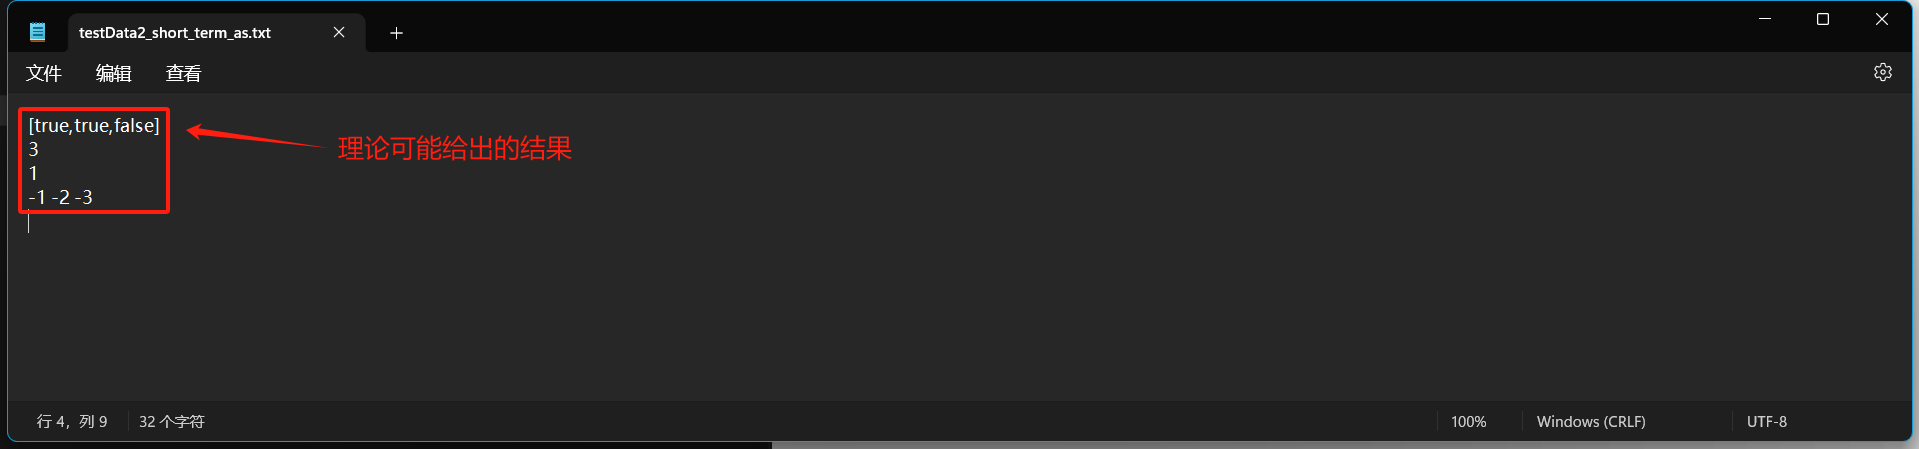
\includegraphics[width=10cm]{Figure/Figure_4.jpg}
        \caption{理论上求解短测例应该得出的结果}
    \end{figure}
    \par
    这是利用回溯法求解短测例给出的结果
    \begin{figure}[H]
        \centering
        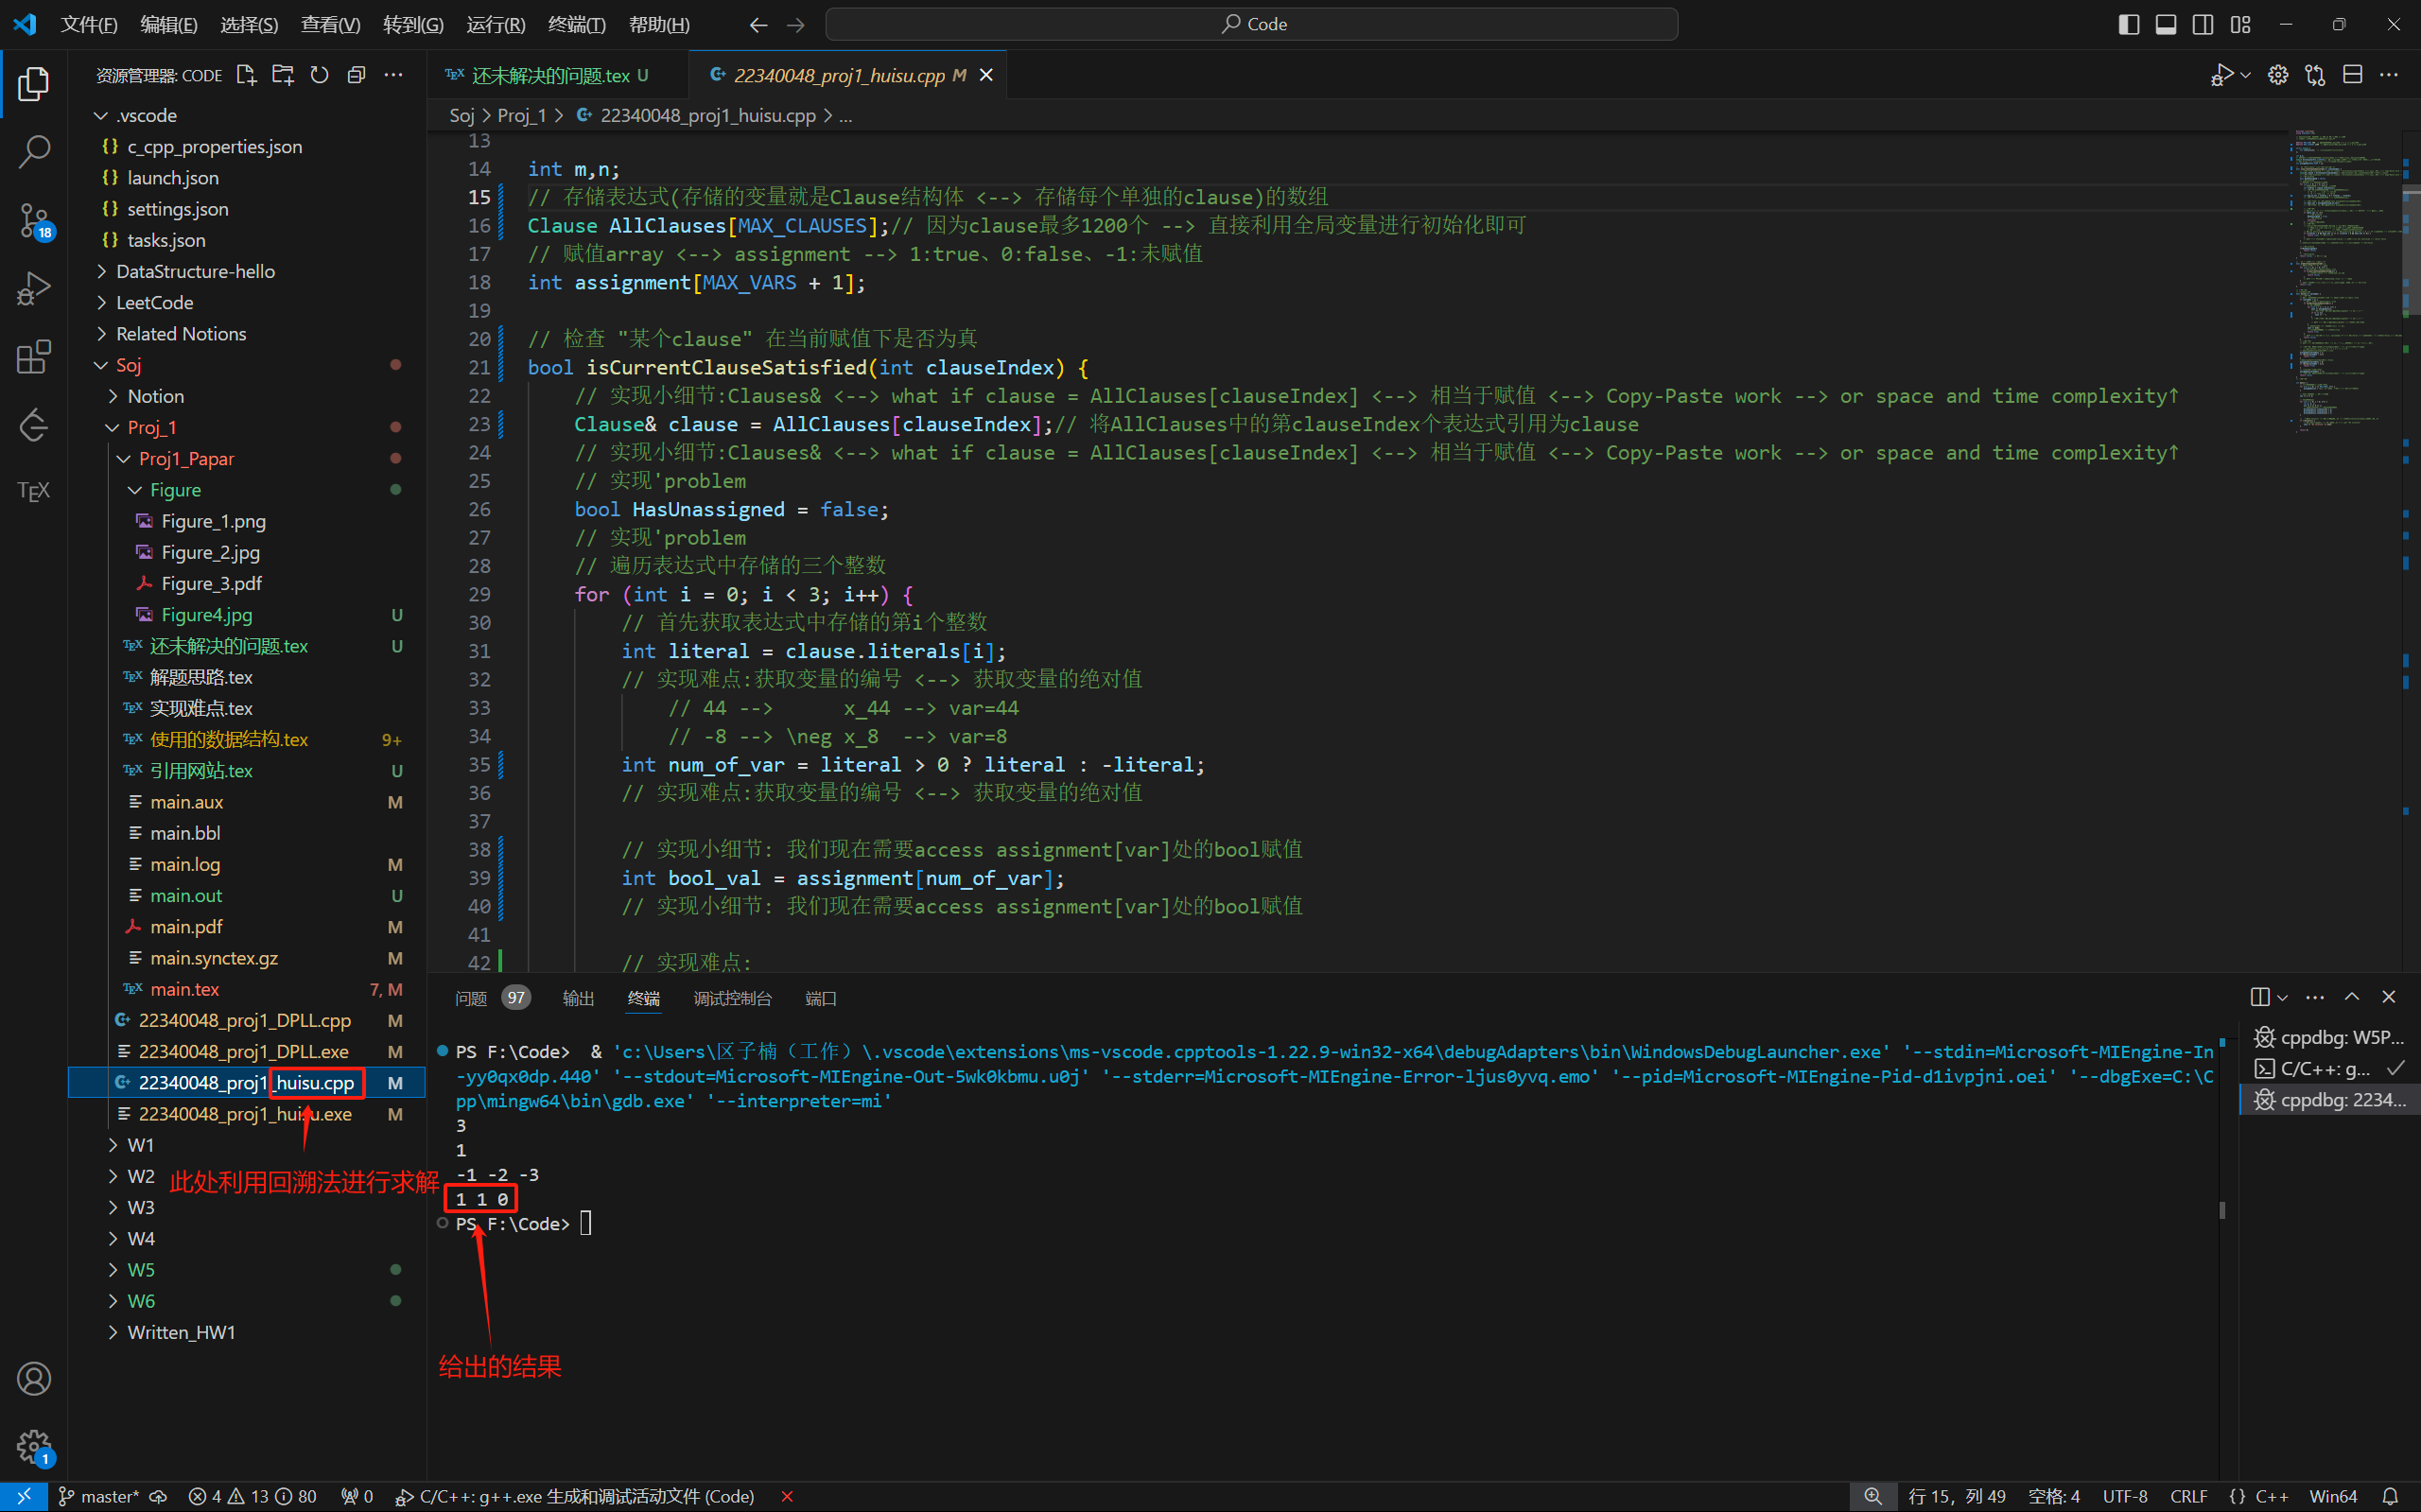
\includegraphics[width=10cm]{Figure/Figure_5.jpg}
        \caption{回溯法求解短测例给出的结果}
    \end{figure}
    \par
    这是利用DPLL算法求解短测例给出的结果
    \begin{figure}[H]
        \centering
        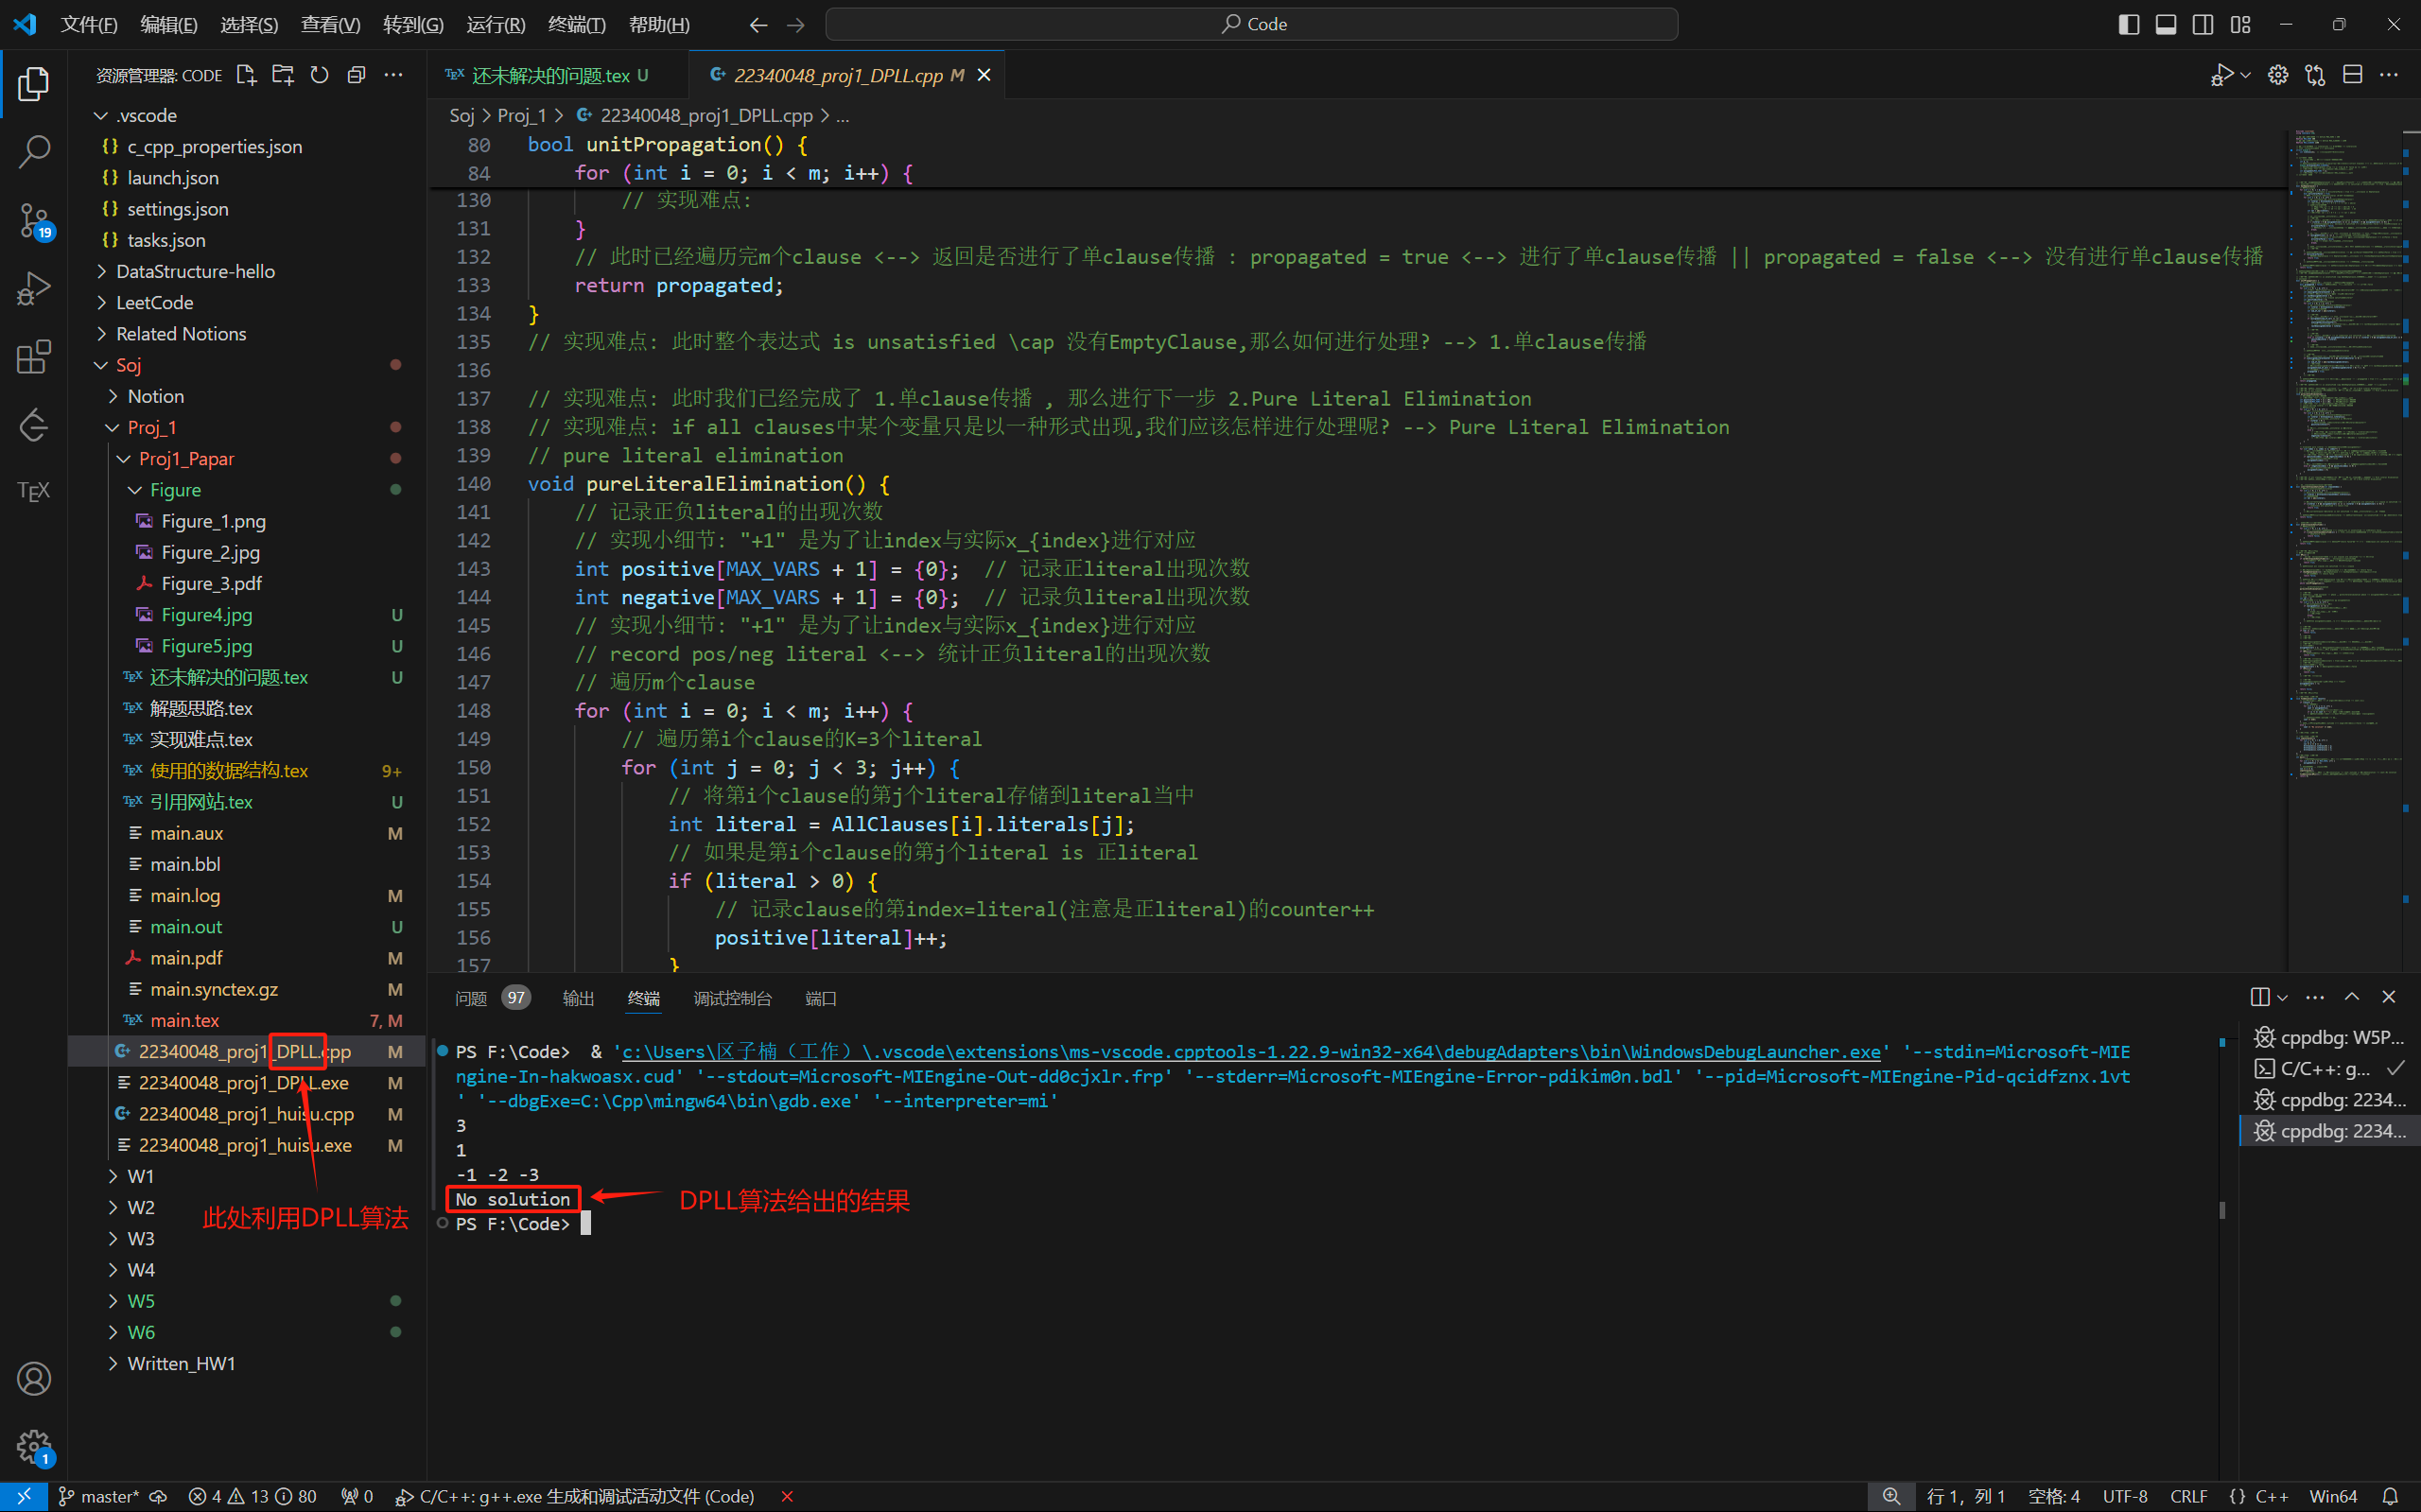
\includegraphics[width=10cm]{Figure/Figure_6.jpg}
        \caption{DPLL算法求解短测例给出的结果}
    \end{figure}
    \par
    很明显现在的这个DPLL算法还是有点小bug的,但是现在还没找出来,留到以后再进行完善。
    \subsection{长测例}
    \par
    考虑如下这么一个例子
    (这里我只放应该得到的结果,实际数据我放在了本地电脑上,如果老师需要我补充数据我也可以提供)
    \begin{figure}[H]
        \centering
        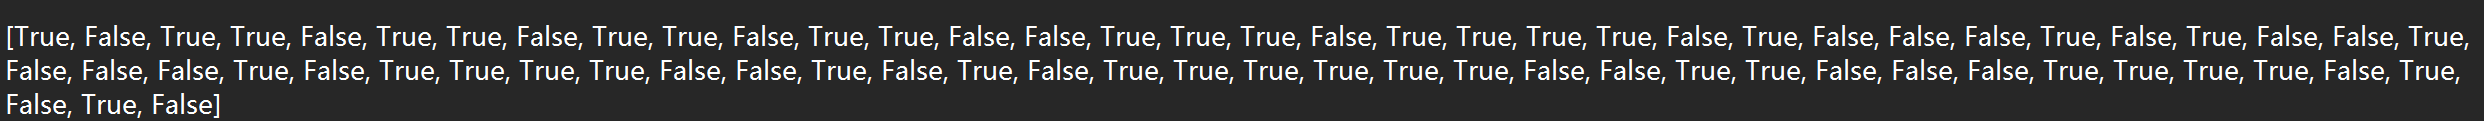
\includegraphics[width=10cm]{Figure/Figure_7.jpg}
        \caption{理论上应该得到的结果}
    \end{figure}
    \par
    这是我利用DPLL算法求解长测例得到的结果
    \begin{figure}[H]
        \centering
        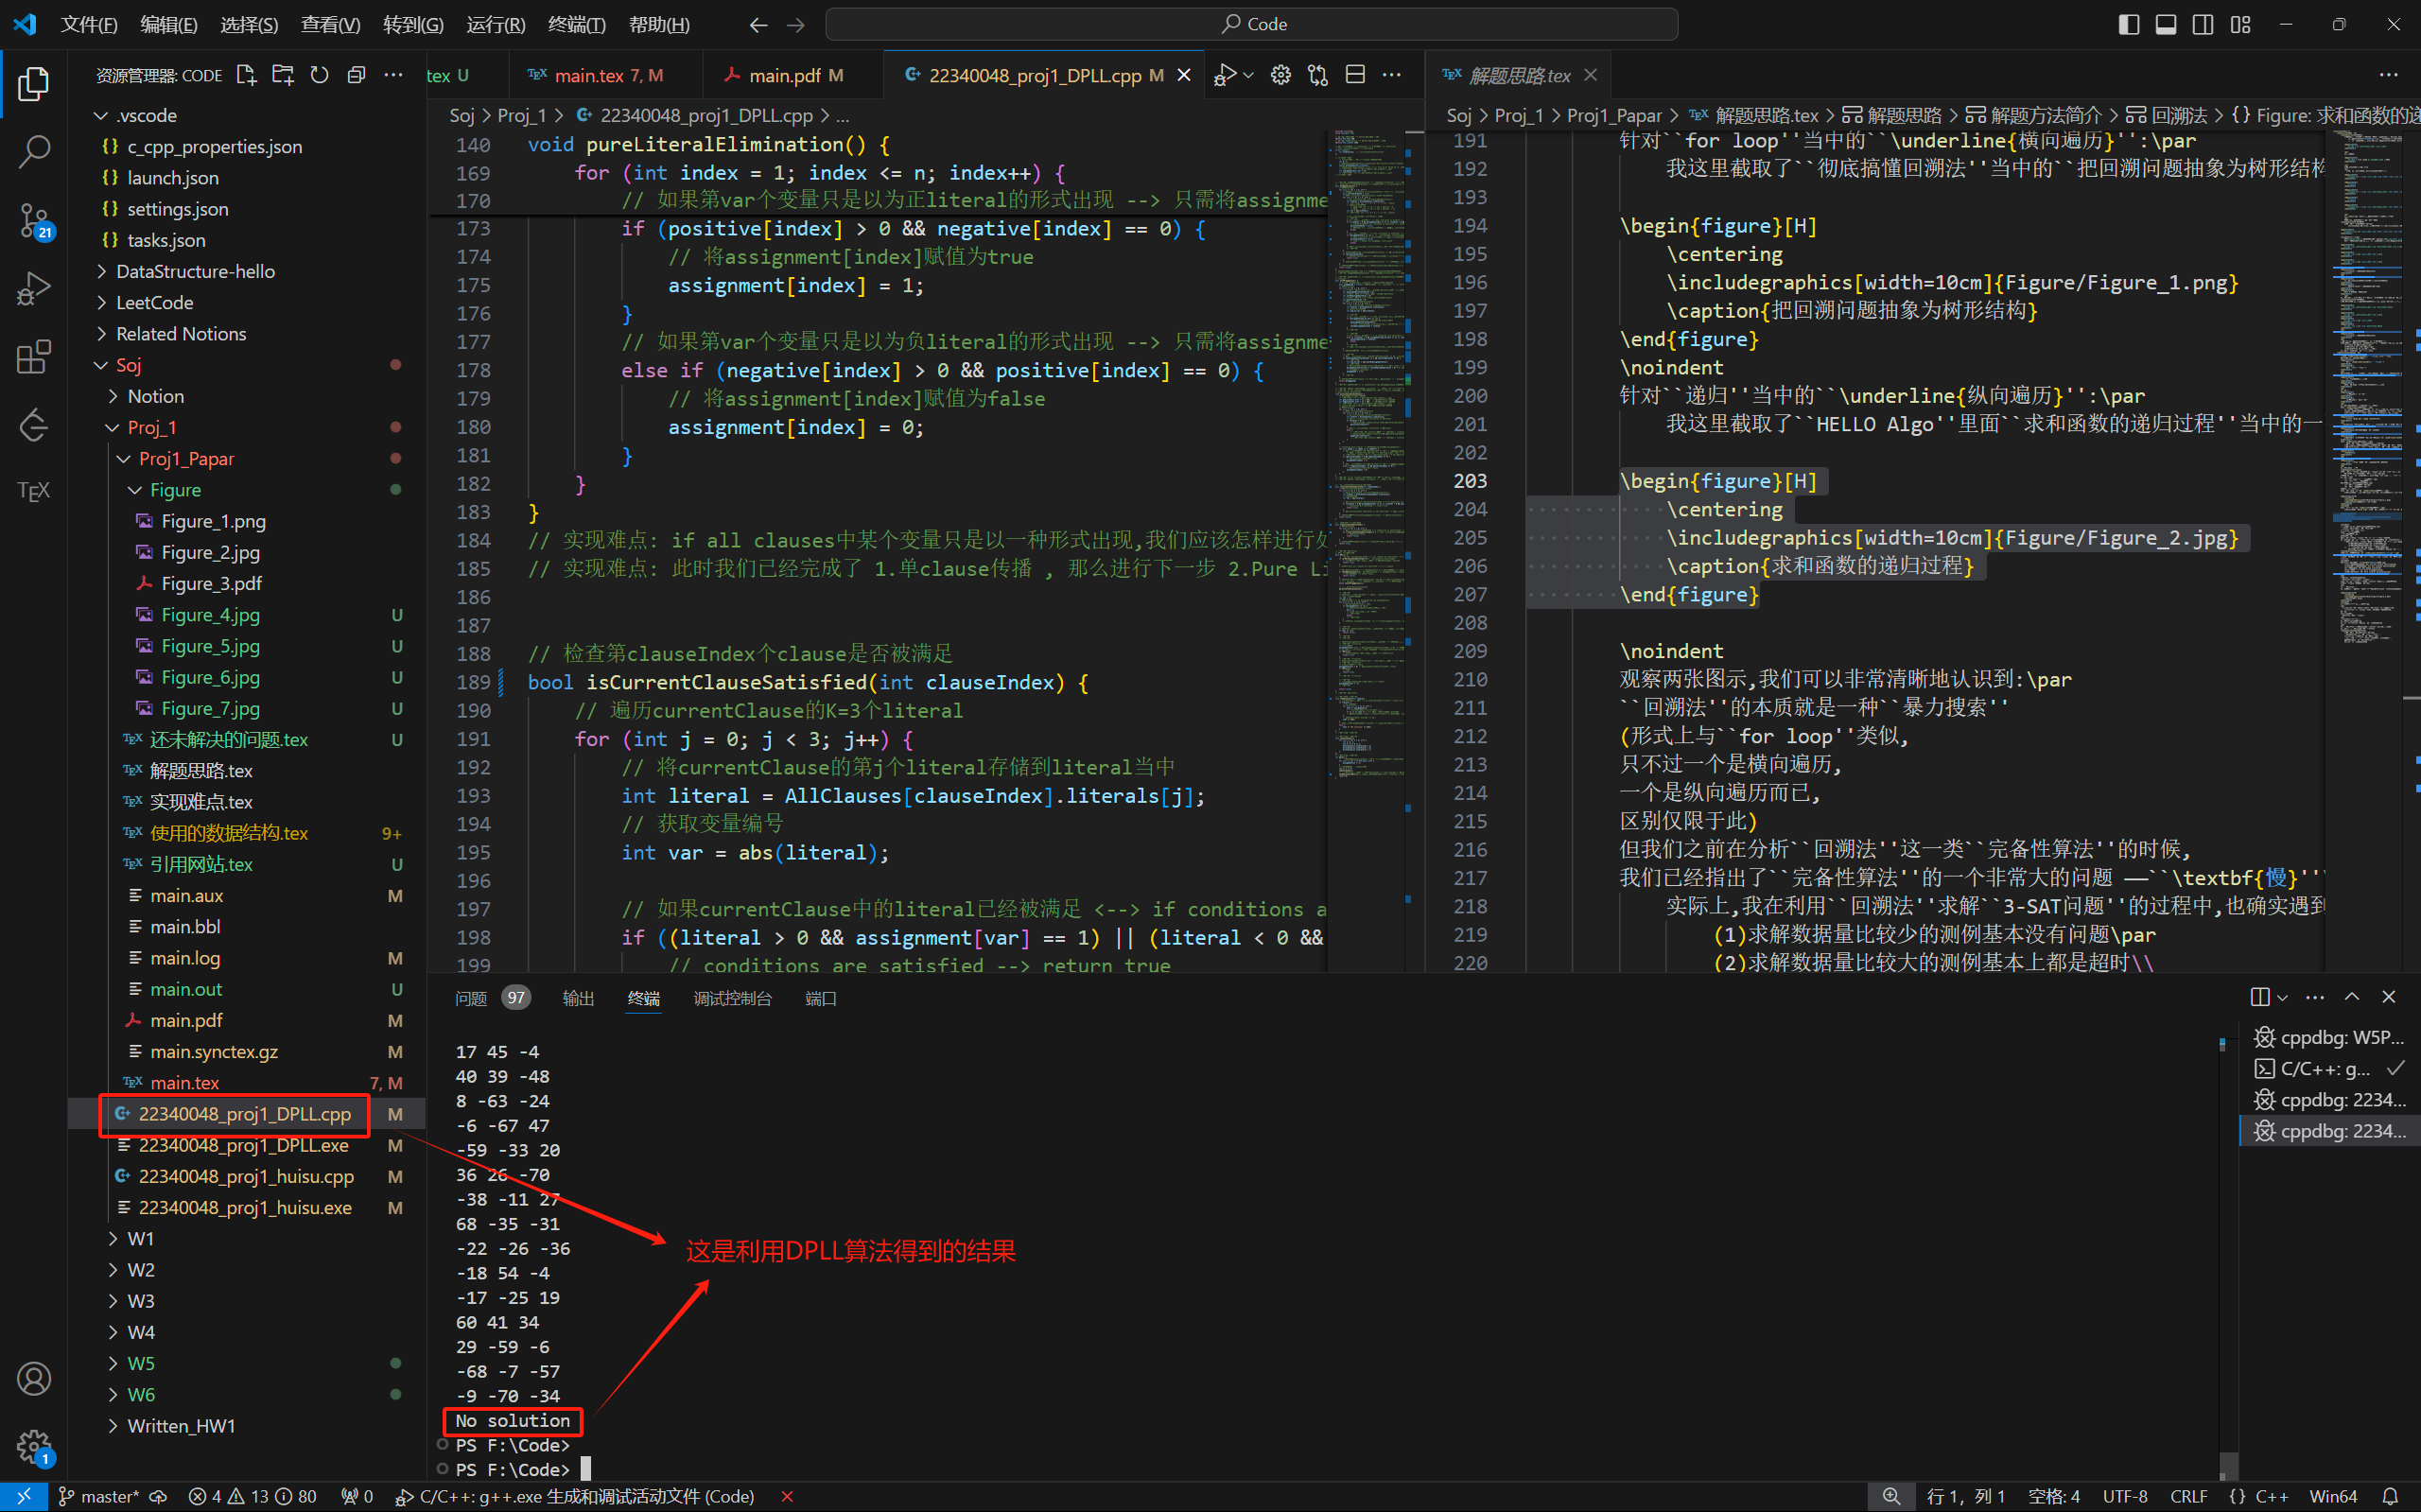
\includegraphics[width=10cm]{Figure/Figure_8.jpg}
        \caption{DPLL算法求解短测例给出的结果}
    \end{figure}
    \par
    同样地,这个长测例也说明了现在的这个DPLL算法还存在一些小漏洞。


\section{引用网站}
\noindent
\href{https://zh.wikipedia.org/wiki/%E5%B8%83%E5%B0%94%E5%8F%AF%E6%BB%A1%E8%B6%B3%E6%80%A7%E9%97%AE%E9%A2%98?oldformat=true}{布尔可满足性问题 - 维基百科}
\newline
\href{https://blog.csdn.net/qaqwqaqwq/article/details/125582233#Boolean_Satisfiability_Problem_SAT_4}{布尔可满足性问题(SAT) - CSDN}
\newline
\href{https://zhuanlan.zhihu.com/p/432853785#:~:text=%E5%8F%AF%E6%BB%A1%E8%B6%B3%E6%80%A7%E9%97%AE%E9%A2%98(Boo)}{SAT问题简介}
\newline
\href{https://zhuanlan.zhihu.com/p/206465770#:~:text=%E7%9B%AE%E5%89%8D%EF%BC%8CSAT%20%E9%97%AE%E9%A2%98%E7%9A%84}{SAT问题的基本概念}
\newline
\href{https://zh.wikipedia.org/wiki/%E5%9B%9E%E6%BA%AF%E6%B3%95}{回溯法(Backtracking) - 维基百科}
\newline
\href{URLhttps://blog.csdn.net/m0_52824954/article/details/123467217}{回溯法 - CSDN}
\newline
\href{https://zh.wikipedia.org/wiki/DPLL%E7%AE%97%E6%B3%95}{DPLL算法(Davis-Putnam-Logemann-Loveland Algo) - 维基百科}
\newline
\href{https://blog.csdn.net/weixin_42695737/article/details/123361318}{DPLL算法 - CSDN}
\newline
\href{https://www.cnblogs.com/chesium/p/15982285.html}{DPLL 算法 - 博客园}
\newline
\href{https://zhuanlan.zhihu.com/p/206710613#:~:text=%E5%BD%93%E5%B1%80%E9%83%A8%E6%90%9C%E7%B4%A2%E5%BA%94%E7%94%A8%E4%BA%8E%E6%B1%82%E8%A7%A3}{局部搜索算法 - 知乎}


\newpage
%--------------------------------------------------参考文献--------------------------------------------------%
\bibliographystyle{plain}                       %表示整体的模板风格
\end{document}                                  %全文结束    
